\section{Effective potential}
The effective potential is a function which to lowest order in pertubation theory is equal to the classical potential energy and to higher orders would include qunatum corrections \cite{Peskin:1995ev}. These corrections are generally not finite and owuld require renormalisation. The effective potential can be used for studying spontaneous symmetry breaking, which is based on minimizing the classical potential $V(\phi)$. However, the vacuum at a qunatum level isn't static, but rather fluctuating. Thus, using the effective potetial these qunatum fluctuation is taken intro account \cite{zee}.
To define the effective potential, we first need to define the effective action. To do this, we consider a scalar field theory $\phi$  with energy as the connected generating functional $E[J]$
\begin{equation}
    Z[J]=e^{-i E[J]}= \int \mathcal{D}\phi\,\phi \exp\left[i\int d^4x (\mathcal{L}[\phi]+J\phi)\right]\;,
\end{equation}
where both the external source $J$ and the field $\phi$ depends on the spacetime coordinate $x$. The equation is in the functional integral formalism. If we translate it to the cannonical formalism we recognize that the right hand side is simply an amplitud on the form
\begin{equation}
    \langle \Omega | \exp\left[-iHT\right] |\Omega\rangle\;,
\end{equation}
where $\ket \Omega$ is the vacuum state of the interacting Hamiltonian $H$, and $T$ is the relevant time interval. Thus, it is simply a vacuum to vacuum amplitude, in the presence of $J$. So $E[J]$ must represent the vacuum energy \cite{Peskin:1995ev}. To define an effective action, we first need to compute the expectation value of the field. This holds information on the state of the vacuum and the systems response to external perturbations
\begin{equation}    
    \phi_{c}(x)\equiv\frac{\delta E[J]}{\delta J(x)}\;,
\end{equation}
the expectation value $\phi_c(x)$ in the canonical formalism $\langle \Omega | \phi(x) |\Omega\rangle_J   $ is a weighted average of the fluctuations of the vacuum configuration and is sometimes called the classical field \cite{Peskin:1995ev}. Now evaluating the functional derivative
\begin{equation}
    \phi_c(x)=-\frac{1}{Z[J]}\int \mathcal{D}\phi\,\phi(x) \exp\left[i\int d^4x (\mathcal{L}[\phi]+J\phi)\right]=\langle \Omega | \phi(x) |\Omega\rangle_J\;.
\end{equation}
Now we can perform a Legendre transformation. This is done analogous to statistical mechanics, where the Legendre transformation relates free energy to the energy: $F = E-TS$, where the free energy is a function of temperature $T$ and the energy is a function of entropy $S$. In this case we have a function $E$ of $J$ and we transform it to the effective action $\Gamma$ which is a function of $\phi_c$\footnote{The difference in parenteses used $()$ and $[]$ refers to the function of or the functional of.}
\begin{equation}
    \Gamma[\phi_c]= -E[J] - \int d^4y\, J(y)\phi_c(y)\;.
    \label{eq:eff pot classical field}
\end{equation}
To better understand the role of the effective action, we take the functional derivative of it with respect to the classical field. This is analogue to the classic action $S[\phi]=\int \text{d}^4 x\, \mathcal{L}(\phi,\partial_\mu\phi)$ where varying the action with respect to the field $\phi(x)\to\phi(x) +\delta \phi(x)$ gives the equations of motion
\begin{equation}
    \frac{\delta S[\phi]}{\delta \phi}=0 \;.
\end{equation}
Now let us do the same for the quantum corrected action
\begin{equation}
    \frac{\delta \Gamma[\phi_c]}{\delta \phi_c(x)}=- \frac{\delta E[J]}{\delta \phi_c(x)} - \int d^4y\,  J(y)\frac{\delta \phi_c(y)}{\delta \phi_c(x)} - \int d^4y\,  \frac{\delta J(y)}{\delta \phi_c(x)}\phi_c(y)\;,
    \label{eq:def of eff pot}
\end{equation}
using the definition of the functional derivative \ref{conventions section} and that $E[J]$ depends on the source, we can rewrite the functional derivative in the first term using the chain rule
\footnote{The chain rule for functional derivatives is a generalization of the standard differentiation chain rule $\frac{\partial f}{\partial x}=\frac{\partial f}{\partial g}frac{\partial g}{\partial x}$ for a composotite function $f(g(x))$. For a functional derivative the difference is that $g(x)\to g_i (\vec x)$. This means that $f$ is a functional of $g$ which is a function of $x$, this is why we consider the continium limit and we have 
\begin{equation*}   
    \frac{\delta f[g]}{\delta g(x)}=\int  \frac{\delta f[g]}{\delta g(x)}\frac{\delta g(x)}{\delta x(y)}
\end{equation*}  
\cite{% https://wiki.physics.udel.edu/wiki_qttg/images/5/53/BOOK%3Ddft_an_advanced_course.pdf p. 411 and https://math.stackexchange.com/questions/235769/is-there-a-chain-rule-for-functional-derivatives 
}
\comment{rewrite this is not super correct} }  
\begin{equation}
    \frac{\delta \Gamma[\phi_c]}{\delta \phi_c(x)}=- \int d^4y\, \frac{\delta J(y)}{\delta \phi_c(x)} \frac{\delta E[J]}{\delta J(y)} - J(x) - \int d^4y\,  \frac{\delta J(y)}{\delta \phi_c(x)}\phi_c(y)\;,
\end{equation}
using the definition of the classical field in Equation \ref{eq:eff pot classical field}, we obtain
\begin{equation}
    \frac{\delta \Gamma[\phi_c]}{\delta \phi_c(x)}=- \int d^4y\, \frac{\delta J(y)}{\delta \phi_c(x)}(-\phi_x(y)) - J(x) - \int d^4y\,  \frac{\delta J(y)}{\delta \phi_c(x)}\phi_c(y)=- J(x)\;.
\end{equation}
Thus, with no external source $J$, the effective action has the same form as the classic action, when computing the equations of motion. The equation can therefore be interpreted as the quantum equation of motion. Using that the effective action, actually is an action we can expand the functional derivative $\Gamma[\phi_c]$
\begin{equation}
    \Gamma[\phi_c] = \int \text{d}^4 x\, \mathcal{L}_{\text{eff}}(\phi_c,\partial_\mu\phi_c)= \int \text{d}^4 x\, \left[-V_{\text{eff}}(\phi_c) + Z(\phi_c)(\partial_\mu \phi_c)^2 + \ddots \right]\;,
\end{equation}
where the $\mathcal{L}_{\text{eff}}$ is the effective lagrangian, $V_{\text{eff}}(\phi_c) $ is the effective potential, and the dots indicate higher powers of derivatives. Using this expansion of the effective action, the functional derivative can aslo be written as
\begin{equation}
    \frac{\delta \Gamma[\phi_c]}{\delta \phi_c(x)}=- \frac{\delta V_{\text{eff}}(\phi_c) }{\delta \phi_c(x)} frac{\delta }{\delta \phi_c(x)}\int \text{d}^4 x\, \left[ Z(\phi_c)(\partial_\mu \phi_c)^2 + \ddots \right]=- \frac{\delta V_{\text{eff}}(\phi_c) }{\delta \phi_c(x)} \;,
\end{equation}
for $\phi_c(x)$ constant in x, and thereby $J$ independent of $x$. Thus, we can write the effective potential as

\begin{equation}
    \frac{\delta V_{\text{eff}}(\phi_c) }{\delta \phi_c(x)} = J(x) \;.
\end{equation}
For the case of no source, the condition that the effective action has an extrenum is converted into a condition on the effective potential to have a minimum \comment{is minimimum correct here? it is not just an extrenum}
\begin{equation}
    \frac{\delta V_{\text{eff}}(\phi_c) }{\delta \phi_c(x)} = 0 \;.
\end{equation}
Consider Equation \ref{eq:def of eff pot} with no source term the vacuum expectation value is determined by minimizing $V_{\text{eff}}$ \cite{zee}.
\comment{I think I need an example of how to calculate it}
\subsection{Calculation of the effective potential}
\begin{equation}
    V_1(h, s) = \sum_i \pm n_i \frac{m_i^4(h, s)}{64\pi^2} \left( \log \left[ \frac{m_i^2(h, s)}{Q^2} \right] - C_i \right)
\end{equation}
and 
\begin{equation}
    V_{\text{eff}}(\varphi) = \frac{\lambda}{4!}\varphi^4 + \frac{\lambda^2 \varphi^4}{256\pi^2} \left( \log \frac{\varphi^2}{Q^2} - \frac{25}{6} \right) + O(\lambda^3)
\end{equation}

For $\ln 2/\lambda =8/3$ and $m^2=\lambda\phi^2/2$

\section{Infinite heat order}
\subsection{Calculations for new paper}

\section{The renormalisation group}



\subsection{The Callan-Symanzik Equation}

\subsection{The beta function and anomalous dimensions}

\subsubsection{An example: Non-Abelian Lagrangian}

\subsection{Fixed point analysis}

\subsubsection{Banks-Zacks fixed point}

So the result is
\begin{equation}
    \beta_{g_{1-loop}}=-\alpha_g^2 b_0 =\frac{-g^3}{16\pi^2}\left[ \frac{11}{3}C_2(H)-\frac{4}{3}n_fC(R)\right]\;.\label{eq:betafunction YM 1loop}
\end{equation}

\section{GUTs}
\subsection{Standard Model}
\subsection{Why GUTs}
\subsection{SU(5)}
\subsection{SO(10)}

\section{CAF analysis}
To constrain the coefficients of the renormalisation equations of a Gauge-Yukawa theory with scalars, we will start by considering a pure gauge theory and working our way to the full model, following a similar approach as \cite{Pica2017ConformalPhase}.  
Consider first the gauge coupling's beta function to one-loop order. 
\begin{equation}
    \mu \frac{\text{d}\alpha_g}{\text{d}\mu}=b_0\alpha_g^2\;,\label{eq:betag1loop}
\end{equation}
where $\mu$ is the energy scale, $\alpha_g=\frac{g^2}{(4\pi)^2}$, and $b_0$ is the coefficient determined by group factors, and the Dynkin index of the representations of the fermions and scalars. We will consider this a constant. For the pure gauge theory to be asymptotically free, we need the beta equation to be negative, that is, $b_0<0$. The solution of the differential equation is
\begin{equation}
    \alpha_g=\frac{\alpha_{g_0}}{1-b_0 \alpha_{g_0} \log \left(\frac{\mu}{\mu_0 }\right)}\;,
    \label{eq:solbetag1loop}
\end{equation}
where the initial condition is $\alpha(\mu_0)=\alpha_{g_0}$. There are three regions to discuss, which are $\mu<\mu_L$, $\mu=\mu_L$, $\mu>\mu_L$, where $\mu_L=\mu_0\exp(\frac1{b_0\alpha_{g_0}})$. In the first case, the logarithm will be negative, and hence the denominator will be negative, because $b_0<0$. In this case, the coupling is negative, and we have an unphysical branch. For the second case, we have a Landaue pole in the infrared. Now, for the final case, the coupling will be positive and will reach asymptotic freedom as $\mu\to\infty$.

Let us now consider the Yukawa coupling's renormalisation equation
\begin{equation}
    \mu \frac{\text{d}\alpha_y}{\text{d}\mu}=\alpha_y(c_1\alpha_g+c_2\alpha_y)\;,\label{eq:betay1loop}
\end{equation}
where $\alpha_y=\frac{y^2}{(4\pi)^2}$, and $c_1$, $c_2$ are constants, where in general $c_1<0$ and $c_2>0$. First, consider the case of no gauge coupling, the solution will be similar to the case of the pure gauge theory
\begin{equation}
    \alpha_y=\frac{\alpha_{y_0}}{1-c_2 \alpha_{y_0} \log \left(\frac{\mu}{\mu_0 }\right)}\;,
\end{equation}
the difference from the previous solution in Equation \ref{eq:solbetag1loop} is that the constant here is positive, so for $\mu\to\infty$ the denominator will be negative, thus this is an unphysical branch. For $\mu<\mu_l$ with $\mu_L=\mu_0\exp(\frac1{c_2\alpha_{y_0}})$ the coupling will be positive. So the coupling will flow to the Gaussian fix point in the infrared and flow towards a Landau pole at high energies. Thus, the Yukawa coupling can never be asymptotically free in the absence of a gauge coupling. 
Let us now consider a theory with both a gauge and a Yukawa coupling:
\begin{align}
    \mu \frac{\text{d}\alpha_g}{\text{d}\mu}&=b_0\alpha_g^2\\\mu \frac{\text{d}\alpha_y}{\text{d}\mu}&=\alpha_y(c_1\alpha_g+c_2\alpha_y)\;,
\end{align}
we now have two coupled differential equations. To solve these, we consider the ratio of the Yukawa and Gauge beta functions
\begin{align}
    \frac{\text{d}\alpha_y}{\text{d}\alpha_g}&=\frac{1}{b_0}\frac{\alpha_y}{\alpha_g}\left(c_1+c_2\frac{\alpha_y}{\alpha_g}\right)\;.\label{eq:betayfrac}
\end{align}
with the solution
\begin{equation}
    \alpha_y=\frac{\alpha_{y_0}}{ \alpha_g^{1-\frac{c_1}{b_0}}\alpha_{g_0}^{\frac{c_1}{b_0}}\left(1-\frac{c_2}{b_0-c_1}\frac{\alpha_{y_0}}{\alpha_{g_0}}\right)+\frac{c_2}{b_0-c_1}\alpha_{y_0} }\alpha_g\;,\quad\quad b_0\neq c_1\;,
\end{equation}
with the initial condition $\alpha_y(\alpha_{g_0})=\alpha_{y_{0}}$. In the case that $b_0=c_1$, the solution changes to 
\begin{equation}
    \alpha_y=\frac{\alpha_{y_0}}{\alpha_{g_0}\left(1+\frac{c_2}{c_1}\frac{\alpha_{y_0}}{\alpha_{g_0}}\log\alpha_{g_0}\right)-\frac{c_2}{c_1}\alpha_{y_0}\log \alpha_g }\alpha_g\;,\quad\quad b_0=c_1\;,\label{eq:ysolb0c1}
\end{equation}
Let us first consider the solution where $b_0=c_1$ in the case of $\alpha_g\to0$. The denominator will be dominated by the second term  $-\frac{c_2}{c_1}\alpha_{y_0}\log \alpha_g $, as the logarithm of the gauge coupling will go towards negative infinity. Since the constant in front will always be negative $\frac{c_2}{c_1}<0$, the $\alpha_y$ coupling will be negative and thus can never be asymptotically free. 
Let us instead consider the first case of $b_0\neq c_1$. The equation can be divided into two parts, one which will be dependent on $\sim\alpha^{\frac{c_1}{b_0}}$ and one $\sim\alpha$. If $\frac{c_1}{b_0}>1$, the first term will dominate, and for $\frac{c_1}{b_0}<1$ the second term will dominate. The case of $\frac{c_1}{b_0}=1$ has already been ruled out from the analysis of Equation \ref{eq:ysolb0c1}. In the case of $\frac{c_1}{b_0}<1$, the coupling will go as \begin{equation}
    \alpha_y\sim\frac{b_0-c_1}{c_2}\alpha_g\;,\quad\quad \frac{c_1}{b_0}<1\;,
\end{equation}
which will always be negative, this can be seen by rewriting the constraint $b_0-c_1<0$. This case will thus not have an asymptotically free Yukawa coupling. The last possible case is the case of $\frac{c_1}{b_0}>1$ or $b_0-c_1>0$. In this case, the coupling will go as
\begin{equation}
    \alpha_y\sim\frac{\alpha_{y_0}}{ \alpha_{g_0}^{\frac{c_1}{b_0}}\left(1-\frac{c_2}{b_0-c_1}\frac{\alpha_{y_0}}{\alpha_{g_0}}\right)}\alpha_g^{\frac{c_1}{b_0}}\;,\quad\quad \frac{c_1}{b_0}>1\;,
\end{equation}
to ensure that the coupling will be positive, we need to constrain the values of the couplings at the arbitrary energy level $\frac{c_2}{b_0-c_1}\frac{\alpha_{y_0}}{\alpha_{g_0}}<1$. In the UV, where $\alpha_g\to 0$, the Yukawa coupling will also be asymptotically free, and because $\frac{c_1}{b_0}>1$, the Yukawa coupling will go faster to zero than the gauge coupling at high energies. Another possibility is that the values of the couplings at the arbitrary energy level are fine-tuned so that $\frac{\alpha_{g_0}}{\alpha_{y_0}}=\frac{c_2}{b_0-c_1}$. In this case, the first term in the denominator vanishes, and the previously dominated term is now the only one left:
\begin{equation}
    \alpha_y=\frac{b_0-c_1}{ c_2 }\alpha_g\;,\quad\quad \frac{\alpha_{g_0}}{\alpha_{y_0}}=\frac{c_2}{b_0-c_1}\;,\quad\quad b_0-c_1>0\;.\label{eq:ygfixed}
\end{equation}
This case is known as fixed flow \cite{SoftenedGravity}. In this case, the Yukawa coupling vanishes at the same order as the gauge coupling. 


The remaining coupling can now be added to the analysis, the self-coupling
\begin{equation}
    \mu \frac{\text{d} \alpha_\lambda}{\text{d}\mu}=\alpha_\lambda\left(d_1\alpha_\lambda + d_2\alpha_g+d_3\alpha_y\right)+d_4\alpha_g^2+d_5\alpha_y^2\;.\label{eq:betalam1loop}
\end{equation}
The coupling is dependent on both the other two couplings, with the coefficients generally $d_1,d_3,d_4\ge0$ and $d_2,d_5\le 0$. Like the two other couplings, we can consider whether the scalar coupling can be asymptotically free on its own. In this case, the solution will be similar to that of the two other couplings
\begin{equation}
    \alpha_\lambda=\frac{\alpha_{\lambda_0}}{1-d_1 \alpha_{\lambda_0} \log \left(\frac{\mu}{\mu_0 }\right)}\;,
\end{equation}
similar to the case of the Yukawa coupling, the constant $d_1$ will be positive. So similar to that case, there will be a Landau pole at the energy scale $\mu_L=\mu_0\exp(\frac1{d_1\alpha_{y_0}})$, where at higher energies than $\mu_L$ the coupling will be negative, for a system with only one scalar couplin,g this must be discarded, since the potential would be unbounded from below. At energies lower than $\mu_,L$, the coupling will be positive with a trivial Gaussian fixed point in the IR. 
Let us now consider a theory with both gauge, Yukawa and scalar coupling. The beta equation of the scalar coupling (Equation \ref{eq:betalam1loop}) can be rewritten similar to Equation \ref{eq:betayfrac} by taking the ratio $\frac{\beta_\lambda}{\beta_g}$
\begin{equation}
    \frac{\text{d} \alpha_\lambda}{\text{d}\alpha_g}=\frac{\alpha_\lambda}{b_0\alpha_g}\left(d_1\frac{\alpha_\lambda}{\alpha_g} + d_2+d_3\frac{\alpha_y}{\alpha_g}\right)+\frac{d_4}{b_0}+\frac{\alpha_y^2}{\alpha_g^2}\;.\label{eq:betalam1loop}
\end{equation}
Recall that the Yukawa coupling can be asymptotically free in two cases, when the Yukawa coupling vanishes faster than the gauge coupling and when they are on fixed flow and go to zero at the same order. Let us start with considering the case of the Yukawa coupling vanishing faster than the gauge coupling, then the differential equations simplify
\begin{equation}
    \frac{\text{d} \alpha_\lambda}{\text{d}\alpha_g}=\frac{\alpha_\lambda}{b_0\alpha_g}\left(d_1\frac{\alpha_\lambda}{\alpha_g} + d_2\right)+\frac{d_4}{b_0}\;.
    \label{eq:betalamfrac}
\end{equation}
with the solution found in Appendix in Equations \ref{eq:alphalamk<0}, \ref{eq:alphalamk>0}, and \ref{eq:alphalamk0} with $k = (b_0 - d_2)^2 - 4d_1 d_4$, and $k_0 = (b_0 - d_2)\alpha_{g_0} - 2d_1\alpha_{\lambda0}$
\begin{align}
    &\alpha_{\lambda} = \frac{\alpha_{g}}{2d_{1}} \left[ b_0 - d_2 + \sqrt{-k} \tan\left( \frac{\sqrt{-k}}{2b_0} \ln\frac{\alpha_g}{\alpha_{g_0}} - \arctan\frac{k_0}{\sqrt{-k\alpha_{g_0}}} \right) \right] , \quad k<0 \\&
    \alpha_{\lambda} = \frac{\alpha_g}{2d_1} \left( b_0 - d_2 - \sqrt{k} \, \frac{ (k_0 + \sqrt{k}\alpha_{g_0}) + (k_0 - \sqrt{k}\alpha_{g_0}) \left( \frac{\alpha_g}{\alpha_{g_0}} \right)^{\sqrt{k}/b_0} }{ (k_0 + \sqrt{k}\alpha_{g_0}) - (k_0 - \sqrt{k}\alpha_{g_0}) \left( \frac{\alpha_g}{\alpha_{g_0}} \right)^{\sqrt{k}/b_0} } \right) , \quad k>0 \label{eq:lambdak>0}\\&
    \alpha_{\lambda} = \frac{ 4b_0 d_1 \alpha_{\lambda0} + k_0 (b_0 - d_2) \ln\frac{\alpha_g}{\alpha_{g_0}} }{ 2b_0 \alpha_{g_0} + k_0 \ln\frac{\alpha_g}{\alpha_{g_0}} } , \quad k=0 \label{eq:lambdak0}
\end{align}
If we start by considering the first solution with $k<0$, the coupling will reach a Landau pole, because of the nature of the tangent function as one varies the gauge coupling. Instead, let us consider the case for $k>0$. From this equation, it can be seen that there are two possible fixed flows between the gauge and self-coupling. Namely, when $k_0+\sqrt{k}\alpha_g=0$ or when $k_0-\sqrt{k}\alpha_g=0$
\begin{equation}
    \alpha_\lambda =\frac{b_0-d_2\pm\sqrt{k}}{2d_1}\alpha_g\;.\label{eq:lamgfixed}
\end{equation}
If we only consider solutions for $\alpha_\lambda>0$ to be relevant solutions, we will see that these fixed flow lines also create the boundaries of the asymptotically free region of the scalar coupling. First, if $\frac{b_0-d_2-\sqrt{k}}{2d_1}>0$, then it is asymptotically free along both fixed flow lines. If $\frac{b_0-d_2+\sqrt{k}}{2d_1}>0$ and $\frac{b_0-d_2-\sqrt{k}}{2d_1}<0$, it will only be asymptotically free along one direction. Lastly, if $\frac{b_0-d_2+\sqrt{k}}{2d_1}<0$, it will not be asymptotically free along any of the fixed flow directions. To ensure that no Landau poles are met within the fixed flow lines, we consider the denominator of Equation \ref{eq:lambdak>0}, to find other possible asymptotically free flows. Take the denominator to be zer,o then the gauge coupling has to uphold
\begin{equation}
    \left(\frac{\alpha_g}{\alpha_{g_0}}\right)^{-\frac{\sqrt{k}}{b_0}}=\frac{k_0+\sqrt{k}\alpha_{g_0}}{k_0-\sqrt{k}\alpha_{g_0}}\;,
\end{equation}
so if there are any solutions, there will be Landau poles. First, the solution of $k_0+\sqrt{k}\alpha_{g_0}=0$ is not relevant, because this zero will be cancelled by a zero in the numerator, as shown by the fixed flow analysis. So for $\alpha_g=0$ there are no Landau poles, however for $\alpha_g>0$ there still might be poles. Since the LHS will be positive, so must the RHS, this means that both the numerator and denominator will have the same sign. Further for $\mu\to \infty$, $\alpha_g\to0$, so that the LHS will be less than one. Essentially, for a pole in the UV, the RHS will have to be less than one, and if the RHS is larger than one, we have a pole in the IR. Thus, for a pole in the UV
\begin{equation}
    0<\frac{k_0+\sqrt{k}\alpha_{g_0}}{k_0-\sqrt{k}\alpha_{g_0}}<1\;,
\end{equation}
For this to be the case, both the denominator and the numerator would have to be negative, for the numerator to be less than the denominator. So to ensure no poles in the UV $k_0+\sqrt{k}\alpha_{g_0}>0$. Considering possible poles in the IR, the condition for a pole will be
\begin{equation}
    1<\frac{k_0+\sqrt{k}\alpha_{g_0}}{k_0-\sqrt{k}\alpha_{g_0}}\;,
\end{equation}
for this to be the case, we need both numerator and denominator to be positive, hence, the numerator needs to be positive for no poles in the UV. We can ensure no poles in the IR by constraining the denominator $k_0-\sqrt{k}\alpha_{g_0}<0$. The reason why we need to have no poles in the IR, even though we are only interested in asymptotic freedom, is that the coupling would blow up at minus infinity, creating an unstable potential. Thus, putting this together with Equation \ref{eq:lamgfixed} the restriction on $\alpha_{\lambda_0}$ and $\alpha_{g_0}$ will be
\begin{equation}
    \frac{b_0-d_2-\sqrt{k}}{2d_1}\le \frac{\alpha_{\lambda_0}}{\alpha_{g_0}}\le \frac{b_0-d_2+\sqrt{k}}{2d_1}\;.
\end{equation}
However, it is also needed to make a further restriction, if at least one of the trajectories has a positive scalar coupling at all scales, this can be done by having a positive upper boundary
\begin{equation}
    {b_0-d_2+\sqrt{k}}>0\;.
\end{equation}
Thus, the self-coupling will be asymptotically free within the boundary of the fixed flow lines and have at least one positive asymptotically free solution for the scalar coupling if
\begin{equation}
    k>0\;,\quad\quad  \frac{b_0-d_2-\sqrt{k}}{2d_1}\le \frac{\alpha_{\lambda_0}}{\alpha_{g_0}}\le \frac{b_0-d_2+\sqrt{k}}{2d_1}, \quad\quad {b_0-d_2+\sqrt{k}}>0\;.
\end{equation}
Now, let us consider the last solution $k=0$. Again, let us consider the denominator to be zero
\begin{equation}
    \ln\frac{\alpha_g}{\alpha_{g_0}}=-\frac{2b_0\alpha_{g_0}}{k_0}\;,
\end{equation}
for $\alpha_g\ge0$, we have again two possible solutions, which will give Landau poles. For $\alpha_g<\alpha_{g_0}$, the RHS has to be negative, for a pole in the UV, so to ensure no poles $k_0>0$. The case will be opposite for the IR, thus $k_0<0$ and the only possible solution inserting this back in Equation \ref{eq:lambdak0}
\begin{equation}
    \alpha_{\lambda} = \frac{ \alpha_{\lambda0}  }{ \alpha_{g_0}  } \alpha_g\;,
\end{equation}
Thus, the restrictions for asymptotically free scalar coupling in this case will be
\begin{equation}
    \alpha_{\lambda} = \frac{ \alpha_{\lambda0}  }{ \alpha_{g_0}  } \alpha_g\;,\quad\quad k_0=0\;, \quad\quad k=0\;
\end{equation}
so in this case, only one flow line would be asymptotically free. 
This was the case of the gauge and Yukawa coupling not on fixed flow, however, for the gauge and Yukawa coupling on fixed flow, the ratio of the beta function of the scalar and gauge coupling doesn't reduce
\begin{equation}
    \frac{\text{d} \alpha_\lambda}{\text{d}\alpha_g}=\frac{\alpha_\lambda}{b_0\alpha_g}\left(d_1\frac{\alpha_\lambda}{\alpha_g} + d_2+d_3\frac{\alpha_y}{\alpha_g}\right)+\frac{d_4}{b_0}+\frac{\alpha_y^2}{b_0\alpha_g^2}\;.
\end{equation}
However, it is not necessary to do the full CAF analysis again for the scalar coupling in this case, because it is possible to remove the Yukawa dependency. This can be done by recalling the fixed flow relation of the Yukawa and gauge coupling in Equation \ref{eq:ygfixed}, so we can replace $\frac{\alpha_y}{\alpha_g}=\frac{b_0-c_1}{c_2}$ 
\begin{equation}
    \frac{\text{d} \alpha_\lambda}{\text{d}\alpha_g}=\frac{\alpha_\lambda}{b_0\alpha_g}\left(d_1\frac{\alpha_\lambda}{\alpha_g} + d_2+d_3\frac{b_0-c_1}{c_2}\right)+\frac{d_4}{b_0}+\frac{(b_0-c_1)^2}{b_0c_2^2}\;.
\end{equation}
Now the equation can be rewritten as
\begin{equation}
    \frac{\text{d} \alpha_\lambda}{\text{d}\alpha_g}=\frac{\alpha_\lambda}{b_0\alpha_g}\left(d_1\frac{\alpha_\lambda}{\alpha_g} + d_2'\right)+\frac{d_4'}{b_0}\;,
\end{equation}
where 
\begin{align}
    d_2'=d_2+d_3\frac{b_0-c_1}{c_2}\;,\quad\quad d_4'&={d_4}+d_5\frac{(b_0-c_1)^2}{c_2^2}\;,
\end{align}
\textcolor{red}{
Obs for these new coefficients, their sign may change? $d_2,d_5\le 0$,  $d_3,d_4\ge0$, and $b_0-c_1>0$ thus
\begin{align}
     &d_2'>0 \quad \text{  if}\quad d_3\frac{b_0-c_1}{c_2}>|d_2|
     \\&d_4'<0 \quad \text{  if}\quad |d_5|\frac{(b_0-c_1)^2}{c_2^2}>d_4
\end{align}
}
thus the solution to the differential equation will be the same as for the case of the Yukawa coupling going to zero faster than the gauge coupling. The constriction on the parameters will also be the same, with $k\to k'=(b_0-d_2')^2-4d_1d_4'$.
After the CAF analysis, we have the following conditions when the Yukawa and gauge couplings are not on fixed flow
\begin{equation}
    b_0<0,\quad\quad b_0-c_1>0,\quad\quad (b_0-d_2)^2-4d_1d_4\geq 0,\quad\quad b_0-d_2+\sqrt{(b_0-d_2)^2-4d_1d_4}>0\;,\label{eq:CAF}
\end{equation}
for the coefficients of the beta functions, and the constraints on the gauge, Yukawa and self-coupling at an arbitrary energy scale 
\begin{align}
    &\text{For }k=0: \quad \alpha_{\lambda} = \frac{ \alpha_{\lambda0}  }{ \alpha_{g_0}  } \alpha_g\;,\quad\quad k_0=0\;.\label{eq:CAFalpha}\\&
    \text{For }k>0: \quad 
    \frac{b_0-d_2-\sqrt{k}}{2d_1}\le \frac{\alpha_{\lambda_0}}{\alpha_{g_0}}\le \frac{b_0-d_2+\sqrt{k}}{2d_1}\;. \label{eq:CAFalphafixed}
\end{align}
Similarly, for a fixed flow condition, the CAF conditions 
\begin{align}
    &b_0<0,\quad\quad b_0-c_1>0,\quad\quad \left(b_0-d_2-d_3\frac{b_0-c_1}{c_2}\right)^2-4d_1\left(d_4+d_5\left(\frac{b_0-c_1}{c_2}\right)^2\right)\geq 0,\\&b_0-d_2- d_3 \frac{b_0-c_1}{c_2}+\sqrt{\left(b_0-d_2 - d_3 \frac{b_0-c_1}{c_2}\right)^2-4d_1\left(d_4+d_5\left(\frac{b_0-c_1}{c_2}\right)^2\right)}>0\;.\label{eq:CAFfixed}
\end{align}  

\section{Chiral theories}
We want to consider chiral theories which are completely asymptotically free. Before doing that, we'll briefly consider what a chiral theory is. Chirality comes from the Dirac equation 
\begin{equation}
    (i\gamma^\mu \partial_\mu - m)\psi (x) =0\;,
\end{equation}
where $\gamma^\mu$ is the gamma matricies. \comment{I use the chiral rep / weyl rep} Rewriting the equation using the momentum operator $\slashed{p}=\gamma^\mu(i\partial_\mu)$ and the $2\times 2$ form of the gamma matricies
\begin{equation}
\left[ 
\begin{pmatrix}
0 & p^0 \\
p^0 & 0
\end{pmatrix}
- 
\begin{pmatrix}
0 & \vec\sigma \cdot \vec p \\
-\vec \sigma \cdot\vec{p}  & 0
\end{pmatrix}
- 
\begin{pmatrix}
m & 0 \\
0 & m
\end{pmatrix}
\right]
\begin{pmatrix}
\psi_L \\
\psi_R
\end{pmatrix}
= 0\;.
\end{equation}
From this it can be seen that massless particles come in two types, left- and right-handed and that they do not mix \cite{for dummies}. In this case an additional symmetry also applies for the field, namely the chiral symmetry $\psi\to e^{i\gamma^5\phi}\psi$ \cite{zee}. Chiral fermions are fermions which transform differently under the gauge group. This also means that you cannot combine left- and right-handed fermions and form a gauge invariant mass term in the lagrangian. Thus, in chiral theories fermions obtain mass at spontantous symmetry breaking like the Higgs mechanism \cite{Peskin:1995ev}.

To investigate chiral theories and how the gauge coupling in the theory change with energy scale, we want to consider the beta function of the lagrangian 
\begin{equation}
    \mathcal{L}=-\frac{1}{4} F^a_{\mu\nu}F^{a\mu\nu} + iT_{ij}\sigma^\mu D_\mu \bar T^{ij} + i\tilde{F}_k\sigma^\mu D_\mu \bar{\tilde{F}}^k+iF_m \sigma^\mu D_\mu \bar{F}^m\;, \label{eq:lagrangian YM Weyl}
\end{equation}
with Weyl fermions in fundamental $F$, anti-fundamental $\tilde{F}$, and two-index symmetric and antisymmetric representations. The lagrangian is thus a Yang-Mills gauge theory with Weyl fermions in different representations. The flavor indices on the anti-fundamental and the fundamental representation is $k=1,2,\ldots,(N\pm 4+p)$ and $m=1,2,\ldots,p$. The interval of these indicies will make sense later. The Weyl fermion representations in the lagrangian are from two chiral theory models. The Georgi-Glashow (anti-symmetric two-index representation) and the Bars-Yankielowicz (symmetric two-index representation) models \cite{M_lgaard_2017}. 

The beta function for Yang-Mills theories to first loop order found in Equation \ref{eq:betafunction YM 1loop}
\begin{equation}
    \beta_{g_{1-loop}}=\frac{-g^3}{16\pi^2}\left[ \frac{11}{3}C_2(H)-\frac{4}{3}n_fC(R)\right]\;,
\end{equation}
this is generic and without a specific fermion representation. First, we want to consider the beta function of the fine structure constant $\alpha_g=\frac{g^2}{16\pi^2}$ instead of the coupling itself
\begin{equation}
    \beta_{\alpha_g}=\frac{\text{d}\alpha_g}{\text{d}\ln \mu}=\frac{2g}{16\pi^2}\frac{\text{d}g}{\text{d}\ln \mu}\;.
\end{equation}
Next we can use that we are considering $\operatorname{SU}(N)$. This results in the Casimir operator $C_2(H)$ to be equal to $N$ \cite{Peskin:1995ev}.\comment{maybe do the calculation earlier}. Thus, the betafunction can be written as
\begin{equation}
    \beta_{\alpha_{g}}={-\alpha_g^2}\left[ \frac{11}{3}N-\frac{4}{3}n_fC(R)\right]\;,
\end{equation}
Next lets consider the second term which depends on the number of fermions for each representation. This is where chiral theories differ from vector-like theories. We consider the same fermionic representations as we had in the lagrangian in Equation \ref{eq:lagrangian YM Weyl}. To do so, it is necessary to specify the flavors of each fermionic representation. This depends on gauge anomalies, also called $\left[\operatorname{SU}(N) \right]^3$ anomalies \cite{Peskin:1995ev}. This anomaly appears in triangle diagrams of three gauge currents. For the theory to be valid the anomaly has to vanish. This happens in the SM. For $\operatorname{SU}(3)_c$ it is trivial because the theory is vector-like and thus have an equal amount of left- and righthanded fermions in the same representation. However, for $\operatorname{SU}(2)_L$ it is not as trivial because it is chiral. For three $\operatorname{SU}(2)_L$ gauge currents the anomaly cancels because the representation is pseudoreal. However, the anomaly can still happen between $\operatorname{SU}(2)_L$ gauge currents and $\operatorname{U}(1)$ or gravity. These combinations still cancel due to the definition of the hypercharge and \comment{why for gravity} \cite{Peskin:1995ev}. 
Thus, to ensure that our chiral theories are anomaly free, it is important that the different representations are build so their anomaly coefficients $A(r)$ cancel
\begin{equation}
    \sum_{fermions}A(r)=\mathcal{A}\overset{!}{=}0\;,
\end{equation}
For a symmetric representation $A(\Psi_{sym})=N+4$ and antisymmetric representation $A(\Psi_{Anti-sym})=N-4$. The fundamental and anti-fundamental representation is given in Equation \ref{eq:anomaly coefficient}. 
\begin{equation}
    \mathcal{A} = N\pm 4 + \bar p A(\bar{\square}) + p A({\square})= N\pm 4 - \bar p  +p= 0 \;,
\end{equation}
where $\bar p$ is the amount of Weyl fermions transforming in the anti-fundamental representation, that is the number of fermion flavors transforming under an anti-fundamental. $p$ is equivalent just for the fundamental representation. Thus, $\bar p$ is restricted to be equal to:
\begin{equation}
    \bar p= N\pm 4 + p  \;.
\end{equation}
Thus, when summing over the Dynkin index for all fermion representations, the anomaly free expression of $\bar p $ is used 
\begin{equation}
    n_f T(R) = T(\Psi) + \bar p T(\bar{\square}) + p T({\square})=\frac{1}{2}\left(N\pm2 + N\pm 4 +p +p\right)=N+p\pm 3\;,
\end{equation}
where $T(\square)=T(\bar \square)$ is given by equation \ref{eq: Dynkin index fund. rep} and $T(\Psi)=\frac{N\pm2}{2}$, where $+$ is for symmetric and $-$ is for anti-symmetric representations. \comment{where does this come from} 
Now inserting this in the beta function, remembering that $n_f$ is the number of Dirac fermions, so we need to divide that term by two, when inserting the amount of Weyl fermions 
\begin{equation}
    \beta_{\alpha_{g}}={-\alpha_g^2}\left[ \frac{22}{3}N-\frac{4}{3}N \mp \frac{12}{3}-\frac{4}{3}p\right]={-\alpha_g^2}\left[ \left(6-\frac{4}{3}x\right)N\mp 4\right]\;,
\end{equation}
where $x=p/N$. From this the fixed point can be found to one loop order by setting the beta function equal to zero as explained in \ref{sec: XX}, yielding two solutions
\begin{equation}
    \beta_{\alpha_{g}}=0\Rightarrow \alpha_g=0 \vee 6N-\frac{4}{3}xN \mp 4=0\;,
\end{equation}
where the first solution is the trivial UV fixed point, also called the gaussian fixed point. The second fixed point is for $x=x_{FP}=\frac{9}{2}\mp \frac{3}{N}$ \cite{M_lgaard_2017} \comment{need to do the fix point analysis - first the veneziano limit takes p and N to infinity but keep x=p/N constant, this makes the explicit chiral factor disappear. I think I need to do the change of variables also for vector like theories to really see the difference.}.

\section{Chiral models with scalars}
\subsection{GG-model with p=0}
Let us start by considering a Georgi-Glashow model \cite{GGmodel}, with transformation properties shown in table \ref{tab:GGp0}. This model has $p=0$, and we will therefore have three fields: the anti-fundamental scalar $\phi$, anti-fundamental fermion $\psi$, and two-index antisymmetric fermion under the gauge group $SU(N)$, where only $\psi$ transforms under the global symmetry group $SU(N-4)$. All fields are charged under the $U(1)$ symmetry.  
\begin{table}[h] 
    \centering 
    \begin{tabular}{|c|c|c|c|c|} \hline Fields & $SU(N)$ & $SU(N-4)$  & $U(1)$ \\ \hline $\Psi$ & $\ytableausetup{boxsize=0.25cm}\begin{ytableau}{}&{}\end{ytableau}$ & 1 & $N-4$ \\ $\psi$ & $\overline\square$ & $\overline\square$ & $-(N-2)$ \\ \hline $\phi$ & $\overline\square$ & 1  & 2 \\ \hline 
    \end{tabular} 
    \caption{Transformation rules of the GG model with $p=0$} 
    \label{tab:GGp0} 
\end{table}
To write the Lagrangian down, we need to ensure that all terms will be invariant under $U(1)$ and that no indices remain open. To do this, we start by writing down the kinetic terms for all particles. Let us first consider the free theory:
\begin{equation}
    \mathcal{L}_{free}= i \bar \Psi_{ij}\sigma^\mu \partial_\mu\Psi_{ij}+i \bar \psi_i^a\sigma^\mu \partial_\mu\psi_i^a+\partial_\mu (\phi^*)_i\partial^\mu\phi_i\;,
\end{equation}
where $\sigma^\mu$ is used because the fermions are chiral and thus are massless. Next, we want to consider the interacting theory, which we do by promoting the global $SU(N)$ symmetry of the Lagrangian to a local symmetry. To ensure gauge invariance we introduce the covariant derivative $\partial_\mu \to D_\mu= \partial_\mu - ie(T^a)^i_{\,j}A_\mu^a$
\begin{equation}
    \mathcal{L}_{kinetic}= -\frac{1}{4} F_{\mu\nu}^a F^{\mu\nu\,a}+i \bar \Psi_{ij}\slashed{D}\Psi_{ij}+i \bar \psi_i^a\slashed{D}\psi_i^a+(D_\mu \phi^*D^\mu\phi)\;,
\end{equation}
where $F_{\mu\nu}^a=\partial_\mu A_\nu^a-\partial_\nu A_\mu ^a+g f^{abc}A_\mu^bA_\nu^c$, with $A_\mu$ being the connection. This gives us our first coupling constant, $g$. If we expand the first term, we get three types of terms
\begin{equation}
    F_{\mu\nu}^a F^{\mu\nu\,a}\approx(\partial_\mu A_\nu^a)^2+ g f^{abc}(\partial_\mu A_\nu^a)A_\mu^bA_\nu^c +g^2 f^{abc}f^{def}A_\mu^bA_\nu^cA_\mu^dA_\nu^e\;,
\end{equation}
which gives us the gauge boson propagator and the two gauge boson vertices. The three remaining kinetic terms give us the scalar and two fermion propagators 
Next, we consider all the possible interaction terms, which we can write in the Lagrangian. Consider first the possible Yukawa interactions. Terms as $\Psi_{ij}\bar A_{ij}H^i$ and $\psi \bar \psi H^i$ are not invariant under $U(1)$. However, mixing the two fermion representations is possible; this, however, gives an open gauge index from the anti-fundamental fermion. Therefore, to have a Yukawa term, we break the global symmetry of $SU(N-4)$. Furthermore, the coupling $y^a$ will thus have the gauge index, giving us $a=N-4$ Yukawa terms, excluding the hermitian conjugate terms.
\begin{equation}
    \mathcal{L}_{Yukawa}= y^a\Psi_{ij} \psi ^a_{\, i} \phi^j + h.c.\; ,
\end{equation}
Lastly, we have to consider possible quartic scalar terms. Again, ensuring $U(1)$ invariant terms, we can write terms like
\begin{align}
    \mathcal{L}_{quartic}= &
    \lambda_1 (\phi^\dagger_i \phi_j)^2 
    + \lambda_2 (\bar \Psi_{ij}\Psi_{ij})^2
    +\lambda_3 (\bar \psi_{i}\psi_{j})^2
    +\lambda_4 (\phi^\dagger_i \phi_j)(\bar \psi_{i}\psi_{j})
    +\lambda_5 (\phi^\dagger_i \phi_j)(\bar \Psi_{ij}\Psi_{ij})
    \\&+\lambda_6 (\bar \psi_{i}\psi_{j})(\bar \Psi_{ij}\Psi_{ij})
    +\lambda_7 (\bar \Psi_{ij}\Psi_{ij})^2+...\;,
\end{align}
and similar terms. However, we will impose another condition, namely that the theory needs to be renormalisable. This means that the coupling should not have negative dimensions. The quartic scalar Lagrangian thus simplifies to one term
\begin{equation}
    \mathcal{L}_{quartic}= 
    \lambda \phi^\dagger_i \phi_i \phi^\dagger_j \phi_j \;,
\end{equation}
thus, we also have one scalar coupling, with the coupling constant $\lambda$. From the quartic and the Yukawa terms, we obtain three new vertices. Before writing up the full Lagrangian, we first consider another possible quartic term 
\begin{align}
    (\phi_i^\dagger T_i ^{\,A\,j}\phi^j)(\phi_k^\dagger T_k ^{\,A\,l}\phi^l)\;.
\end{align}
However, for (anti-)fundamental representations, it is not linearly independent on the quartic scalar term $\lambda \phi^\dagger_i \phi_i \phi^\dagger_j \phi_j $  already written. This can be proved by considering that the generators $T^A$ uphold the Fierz identity
\begin{align}
    T_i ^{\,A\,j}T_k ^{\,A\,l}=\frac{1}{2}\left(\delta_i^{\,l}\delta_k^{\,j}-\frac{1}{N}\delta_i^{\,j}\delta_k^{\,l}\right) \;.
\end{align}
The Fierz identity can be shown to be true for fundamental representations of $SU(N)$ by considering the trace of the generators. The generators of $SU(N)$ can be written as $n\times n $ traceless Hermitian matrices $T^a$. The normalisation of these matrices is first defined to be 
\begin{equation}
      \text{tr}(T^a T^b)=\frac{1}{2}\delta^{ab}\;,
\end{equation}
using this, we can write a general matrix $M$ as a linear combination of the identity matrix and the generators of the Lie algebra
\begin{equation}
      M=n_0 I+n_aT^a\;,
\end{equation}
where $n_0$ and $n_a$ are coefficients. Now let us take the trace on both sides and simplify using that $\tr(T^a)=0$ and $\tr(I)=N$
\begin{equation}
      \tr(M)=n_0 \tr(I)+n_a\tr(T^a)=n_0N\;.\label{eq:tr1}
\end{equation}
Next, using the definition of the normalisation of the generators
\begin{equation}
      \tr(MT^b)=n_0 \tr(IT^b)+n_a\tr(T^aT^b)=\frac{n_b}{2}\;.\label{eq:tr2}
\end{equation}
Now using Equation \ref{eq:tr1,eq:tr2}, the constants $n_0,n_a$ can be replaced, and the matrix $M$ can be written as
\begin{equation}
      M=\frac{\tr(M)}{N} I+2\tr(MT^a)T^a\;,
\end{equation}
the matrix decomposition can be written in index notation
\begin{equation}
      M_{ij}=\frac{\tr(M)}{N} \delta_{ij}+2\tr(MT^a)T^a_{ij}\;,
\end{equation}
Using that it is in Euclidean space with the metric $\delta_{ij}$, the traces can be simplified, and the lhs can be rewritten
\begin{equation}
      \delta_{jk}\delta_{il}M_{lk}=\frac{1}{N} \delta_{kl}M_{lk}\delta_{ij}+2\delta_{ln}M_{lk}T^a_{kn}T^a_{ij}\;,
\end{equation}
which can be simplified to 
\begin{equation}
      \delta_{jk}\delta_{il}=\frac{1}{N} \delta_{kl}\delta_{ij}+2T^a_{kl}T^a_{ij}\;,
\end{equation}
Isolating 
\begin{equation}
      T^a_{kl}T^a_{ij}=\frac{1}{2}\left(\delta_{jk}\delta_{il}-\frac{1}{N} \delta_{kl}\delta_{ij}\right)
\end{equation}
Inserting this back into the term gives us
\begin{align}
    \frac{1}{2} (\phi_i^\dagger \phi^j)(\phi_k^\dagger \phi^l)\left(\delta_i^{\,l}\delta_k^{\,j}-\frac{1}{N}\delta_i^{\,j}\delta_k^{\,l}\right)=\frac{1}{2}\left[\phi^{\dagger}_i \phi^j \phi^{\dagger}_j \phi^i-\frac{1}{N}\phi^{\dagger}_i \phi^i \phi^{\dagger}_k \phi^ik\right]=\frac{1}{2}\left(1-\frac{1}{N}\right) (\phi^{\dagger}_i \phi^i))^2\;,
\end{align}
so it is not linearly independent of the quartic term in the Lagrangian. Thus, the full Lagrangian reads
\begin{equation}
    \mathcal{L}= -\frac{1}{4} F_{\mu\nu}^a F^{\mu\nu\,a}+i \bar \Psi_{ij}\slashed{D}\Psi_{ij}+i \bar \psi_i^a\slashed{D}\psi_i^a+(D_\mu \phi^*D^\mu\phi)^2+(y^a\Psi_{ij} \psi ^a_{\, i} \phi^j + h.c.)+\lambda \phi^\dagger_i \phi_i \phi^\dagger_j \phi_j 
    \;.
\end{equation}

\subsubsection{Beta functions of the Lagrangian}
To analyse whether the theory is asymptotically free, we will use the Callan-Symanzik Equation. The beta function will first be computed for the gauge coupling
\begin{equation}
    \beta(g)=\mu\frac{\text{d}g}{\text{d}\ln\mu}= b_0 g^3\;,
\end{equation}
where $\mu$ is an arbitrary energy scale. The beta function with Weyl fermions and complex scalars is given by \cite{betafunctionstwoloop}
\begin{equation}
    \beta(g)=-\frac{g^3}{(4\pi)^2}\left[\frac{11}{3}C_2(G)-\frac{2}{3}T(F)-\frac{1}{3}T(S)\right]\;,\label{eq:betag1loop}
\end{equation}
for the considered GG-model the quadratic Casimir $C_2(G)=N$ and the Dynkin index $T(F)_\Psi=\frac{N-2}{2},\, T(F)_\psi=\frac{1}{2}, \, T(S)_\phi=\frac{1}{2}$ can be inserted
\begin{align}
    \beta(g)=&-\frac{g^3}{(4\pi)^2}\left[\frac{11}{3}N-\frac{2}{3}\left(\frac{N-4}{2}+\frac{N-2}{2}\right)-\frac{1}{6}\right]
    \\=&-\frac{g^3}{(4\pi)^2}\left[3N+\frac{11}{6}\right]\;.
\end{align}
Defining the coupling as $\alpha_g=\frac{g^2}{4\pi}$, the beta function reduces to
\begin{align}
    \beta(\alpha_g)=-\frac{\alpha_g^2}{6}\left[N+22\right]\;.
\end{align}
The remaining beta function is computed using the "RGBeta" library in Mathematica \cite{Thomsen2021RGBeta}.
When computing the beta function for the Yukawa and the scalar coupling, the terms dependent on the Yukawa coupling are not completely trivial. They will have an index, because the coupling has the $a$ index, for the beta function of the Yukawa coupling
\begin{align}
    \beta_{y}\sim c_1g^2y_i + c_2 y^T \bar y y_i\;, 
\end{align} 
where the last term
\begin{equation}
    y^T \bar y =\sum_k^M y_k y_k^*=\sum^M_k |y_k|^2\;,
\end{equation}
for all Yukawas equal, this reduces to
\begin{equation}
   \sum^M_k |y_k|^2=My^2\;,
\end{equation}
Only the terms with $y^3$ will be affected by the $M=N\pm4 +p$ factor. Thus, only the prefactors $c_2\to M c_2$,  $d_3\to M d_3$ and  $d_5\to M^2 d_5$. This, however, does not change the CAF condition, not on Fixed flow, hence none of the coefficients take part in the conditions. However, for fixed flow conditions, the CAF conditions include all coefficients
\begin{align}
    &b_0<0,\quad\quad b_0-c_1>0,\quad\quad \left(b_0-d_2-Md_3\frac{b_0-c_1}{Mc_2}\right)^2-4d_1\left(d_4+M^2d_5\left(\frac{b_0-c_1}{Mc_2}\right)^2\right)\geq 0,\\&b_0-d_2- Md_3 \frac{b_0-c_1}{Mc_2}+\sqrt{\left(b_0-d_2 - Md_3 \frac{b_0-c_1}{Mc_2}\right)^2-4d_1\left(d_4+M^2d_5\left(\frac{b_0-c_1}{Mc_2}\right)^2\right)}>0\;.
\end{align}  
For these CAF conditions, the additional factor of $M$ from the Yukawa coupling cancels out, and therefore does not affect whether the theory is CAF or not. 
The index on the Yukawa coupling can also be simplified by using that $y_ay^a=y^2$, i.e. treating $y_a$ as a vector which can be rotated along any basis under an $SU(N-4)$ transformation, so that it can be written as a vector with only one entry, the first as $y$. The beta functions for the self-coupling and the Yukawa coupling are then
\begin{align}
    \beta_{\alpha_y}&= \frac{\alpha_y }{2}\left[(3 N-1)
   \alpha_y+6 \alpha_g \left(-3 N+2+\frac 5N\right)\right]\\
    \beta_{\alpha_\lambda}&=\alpha_\lambda\left[2(N+1)\alpha_y-\frac{6 \alpha_g \left(N^2-1\right)}{N}+4 \alpha_\lambda (N+4)\right]-\frac{1}{2} (N+3)\alpha_y^2+\frac{3 \alpha_g^2 \left(N^3+N^2-4 N+2\right)}{4 N^2} 
\end{align}
Before diving into the CAF analysis of this model, let us consider a similar model.
\subsection{BY-model with p=0}
\begin{table}[h] 
    \centering 
    \begin{tabular}{|c|c|c|c|c|} \hline Fields & $SU(N)$ & $SU(N+4)$  & $U(1)$ \\ \hline $\chi$ & $\ytableausetup{boxsize=0.25cm}\begin{ytableau}{}\\{}\end{ytableau}$ & 1 & $N+4$ \\ $\psi$ & $\overline\square$ & $\overline\square$ & $-(N+2)$ \\ \hline $\phi$ & $\overline\square$ & 1  & -2 \\ \hline 
    \end{tabular} 
    \caption{ Transformation rules of the BY-model with $p=0$} 
    \label{tab:BYp0} 
\end{table}
Considering a chiral model with scalars, we now focus on the Bars-Yankielowicz model \cite{Bars1981BY}. As seen in table \ref{tab:BYp0}, the main difference from the GG-model is that instead of having a two-index antisymmetric representation, we have a two-index symmetric representation. That is the fermionic field $\chi_{ij}=\chi_{ji}$. The Lagrangian is similar to that of the GG-model and can be expressed as
 \begin{align*}\mathcal{L}= -\frac{1}{4} F_{\mu\nu}^a F^{\mu\nu\,a}+i \bar \chi^{ij}\slashed{D}\chi_{ij}+i \bar \psi_{i\,a}\slashed{D}\psi_i^a+(D_\mu \phi^{*\,i})(D^\mu\phi_i)+(y^a\chi^{ij} \psi ^a_{\, i} \phi_j + h.c.)+\lambda (\phi^{\dagger}_i \phi^i)( \phi^{\dagger}_j \phi^j )
    \;.
 \end{align*}
 where the gauge beta function can be found similar to the GG-model, with the only change in the number of $\psi$ fermions being $N+4$ and the Dynkin index of $T(F)_\Psi=\frac{N+2}{2}$
 \begin{align}
    \beta(g)=&-\frac{g^3}{(4\pi)^2}\left[\frac{11}{3}N-\frac{2}{3}\left(\frac{N+4}{2}+\frac{N+2}{2}\right)-\frac{1}{6}\right]
    \\=&-\frac{g^3}{(4\pi)^2}\left[3N-\frac{13}{6}\right]\;.
\end{align}
Making a change of variables using
\begin{align}
    \alpha_g = \frac{g^2}{(4\pi)^2}, \quad \alpha_y = \frac{y^2}{(4\pi)^2}, \quad\alpha_\lambda = \frac{\lambda}{(4\pi)^2}
\end{align}
We obtain the beta functions
\begin{align}
 \beta_{\alpha_g}&=-\frac{-13+18N}{3}\alpha_g^2\\
    \beta_{\alpha_y}&= \frac{\alpha_y}{2}\left[(3 N+5)\alpha_y+6 \alpha_g\left(-3 N-2+\frac 5N\right) \right]
   \\
   \beta_{\alpha_\lambda}&=\alpha_\lambda\left[2(N+1)\alpha_y-\frac{6 \alpha_g 
   \left(N^2-1\right)}{N}+4 \alpha_\lambda (N+4)\right]-\frac{1}{2} (N+3)
  \alpha_y^2+\frac{3 \alpha_g^2 \left(N^3+N^2-4 N+2\right)}{4 N^2} 
\end{align}
Before doing the CAF analysis, we can check that in the large $N$ limit, the beta functions of the two models should agree. We can write the beta functions as:
\begin{align}
    \beta(\alpha_g)&=-\frac{\alpha_g^2}{3}\left[18N\pm{12}-1\right]\;, \label{eq:GGBYp0betag}\\
    \beta_{\alpha_y}&= \frac{\alpha_y}{2}\left[(3 N+2\mp3)\alpha_y+6 \alpha_g\left(-3 N\pm2+\frac 5N\right) \right]
  \label{eq:GGBYp0betay} \\
   \beta_{\alpha_\lambda}&=\alpha_\lambda\left[2(N+1)\alpha_y-\frac{6 \alpha_g 
   \left(N^2-1\right)}{N}+4 \alpha_\lambda (N+4)\right]-\frac{1}{2} (N+3)
  \alpha_y^2+\frac{3 \alpha_g^2 \left(N^3+N^2-4 N+2\right)}{4 N^2} \;,\label{eq:GGBYp0betas}
\end{align}
where the upper sign belongs to the GG-model and the lower sign to the BY-model. For large N, both models reduce to
\begin{align}
    \beta_{\alpha_g}&\approx-6N\alpha_g^2\\
    \beta_{\alpha_y}&\approx N\alpha_y\left(-9\alpha_g+\frac{3}{2}\alpha_y\right)\\
    \beta_{\alpha_\lambda}&\approx N\left(\alpha_\lambda\left[2\alpha_y-6 \alpha_g 
   +4 \alpha_\lambda \right]-\frac{1}{2}
  \alpha_y^2+\frac{3}{4} \alpha_g^2 \right)\;.
\end{align}
Now, we can investigate whether for any N the model is completely asymptotically free. 
\subsection{CAF analysis of the GG and BY model with $p=0$}
From the CAF conditions in Equation \ref{eq:CAF} and \ref{eq:CAFfixed}, restrictions can be made on values of $N$. This can be seen in Figure \ref{fig:p0}. As the figure shows, no values of $N$, make the couplings asymptotically free when the gauge and the Yukawa couplings are not on fixed flow (Equation \ref{eq:ygfixed}). Only on a fixed flow is there a possibility for CAF. The same applies to both the GG- and BY-models. For the GG-model, $N\ge8$ and for the BY model, $N\ge2$.
\begin{figure}[h]
    \centering
    \begin{subfigure}{0.45\textwidth}
        \centering
        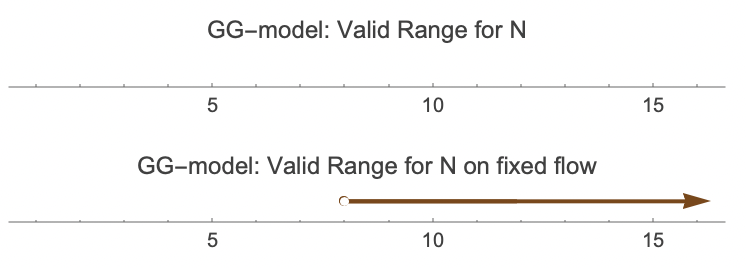
\includegraphics[width=\linewidth]{Figures/GGp0.png}
        %\caption{} % optional subcaption
        \label{fig:GGp0}
    \end{subfigure}
    \hfill
    \begin{subfigure}{0.45\textwidth}
        \centering
        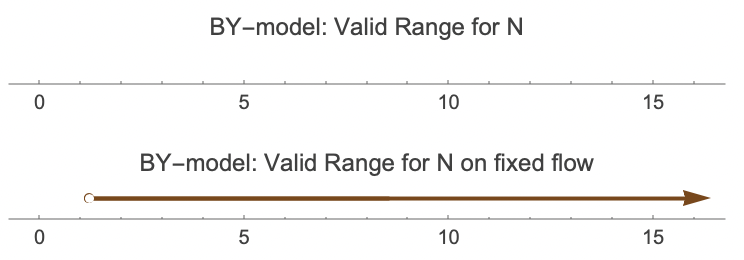
\includegraphics[width=\linewidth]{Figures/BYp0.png}
        %\caption{} % optional subcaption
        \label{fig:BYp0}
    \end{subfigure}
    \caption{The figures show values of N (dark brown), which fulfil conditions for CAF. The upper plots show solutions for gauge and Yukawa coupling not on a fixed flow. The lower plots show on fixed flow. To the left is the GG-model, to the right the BY-model.}
    \label{fig:p0}
\end{figure}


\subsection{GG and BY models with $p\neq0$}
\begin{table}[h]
    \centering
    \begin{tabular}{|c|c|c|c|c|c|}
    \hline
    Fields & $SU(N)$ & $SU(N - 4 + p)$ & $SU(p)$ & $U_1(1)$ & $U_2(1)$ \\
    \hline
    $\Psi$ & $\ytableausetup{boxsize=0.25cm}\begin{ytableau}{}\\{}\end{ytableau}$ & $1$ & $1$ & $N - 4$ & $2p$ \\

    $\tilde\psi$ & $\overline\square$ & $\overline\square$ & $1$ & $-(N - 2)$ & $-p$ \\

    $\psi$ & $\square$ & $1$ & $\square$ & $N - 2$ & $-(N - p)$ \\
    \hline
    $\phi$ & $\overline\square$ & $1$ & $1$ & $2$ & $-p$ \\
    \hline
    \end{tabular}
    \caption{Transformation rules of the GG-model with $p\neq 0$ } 
    \label{tab:GGp} 
\end{table}


\begin{table}[h]
    \centering
    \begin{tabular}{|c|c|c|c|c|c|}
    \hline
    Fields & $[SU(N)]$ & $SU(N + 4 + p)$ & $SU(p)$ & $U_1(1)$ & $U_2(1)$ \\
    \hline
    $\chi$ & $\ytableausetup{boxsize=0.25cm}\begin{ytableau}{}&{}\end{ytableau}$ & $1$ & $1$ & $N + 4$ & $2p$ \\

    $\tilde\psi$ & $\overline\square$ & $\overline\square$ & $1$ & $-(N + 2)$ & $-p$ \\

    $\psi$ & $\square$ & $1$ & $\square$ & $N +2$ & $-(N - p)$ \\
    \hline
    $\phi$ & $\overline\square$ & $1$ & $1$ & $-2$ & $-p$ \\
    \hline
    \end{tabular}
    \caption{Transformation rules of the BY-model with $p\neq 0$ } 
    \label{tab:BYp} 
\end{table}
A second set of models we will consider is the GG- and BY-Model with $p\neq0$, we will see that these have the possibility of being CAF for certain $N,p$, even if the Yukawa and scalar coupling are not on fixed flow. First, the model considered is similar to the ones with $p=0$, i.e., having one scalar in the anti-fundamental representation. The transformation table changes a bit (see Table \ref{tab:GGp} and \ref{tab:BYp}), however the lagrangian will be similar
\begin{equation}
    \mathcal{L}= -\frac{1}{4} F_{\mu\nu}^a F^{\mu\nu\,a}+i \bar \Psi_{ij}\slashed{D}\Psi_{ij}+i \bar \psi_i^a\slashed{D}\psi_i^a+i \bar {\tilde \psi}_i^a\slashed{D}\tilde\psi_i^a+(D_\mu \phi^*D^\mu\phi)^2+(y^a\Psi_{ij} \tilde\psi ^a_{\, i} \phi^j + h.c.)+\lambda (\phi^\dagger_i \phi_i)^2 
    \;,
\end{equation}
where the kinetic term for the $\tilde\psi$ has been added. Only the one Yukawa term can be written down, for the Lagrangian to be invariant under both $U_1(1)$ and $U_2(1)$. The beta functions of the models will also be similar to beta equations in Equation \ref{eq:GGBYp0betag}, \ref{eq:GGBYp0betay}, and \ref{eq:GGBYp0betas}. The only change will be to the gauge beta function, because the amount of fermions affects the $b_0$ coefficient. Using the Equation \ref{eq:betag1loop}, we can compute the gauge beta function
\begin{equation}
    \beta(\alpha_g)=-{2\alpha_g^2}\left[\frac{11}{3}C_2(G)-\frac{2}{3}T(F)-\frac{1}{3}T(S)\right]\;,
\end{equation}
where $C_2(G)=N, \,T(F)_\Psi=\frac{N\mp2}{2},\, T(F)_\psi=\frac{1}{2},\, T(F)_{\tilde\psi}=\frac{1}{2},\, T(S)_\phi=\frac{1}{2}$ inserting this we obtain
\begin{equation}
    \beta(\alpha_g)=-{2\alpha_g^2}\left[\frac{22}{6}N-\frac{2}{3}\left(\frac{N\mp4+p}{2}+\frac{p}{2}+\frac{N\mp2}{2}\right)-\frac{1}{6}\right]\;,
\end{equation}
\begin{equation}
    \beta(\alpha_g)=-\frac{\alpha_g^2}{3}\left[18N-4p\pm{12}-1\right]\;,\label{eq:betagwithp}
\end{equation}
where the two remaining beta functions are given by
\begin{align}
    \beta_{\alpha_y}&= \frac{\alpha_y}{2}\left[(3 N+2\mp3)\alpha_y+6 \alpha_g\left(-3 N\pm2+\frac 5N\right) \right]\label{eq:betaywithp}
   \\
   \beta_{\alpha_\lambda}&=\alpha_\lambda\left[2(N+1)\alpha_y-\frac{6 \alpha_g 
   \left(N^2-1\right)}{N}+4 \alpha_\lambda (N+4)\right]-\frac{1}{2} (N+3)
  \alpha_y^2+\frac{3 \alpha_g^2 \left(N^3+N^2-4 N+2\right)}{4 N^2} \label{eq:betalamwithp}
\end{align}
\begin{figure}[h]
    \centering
    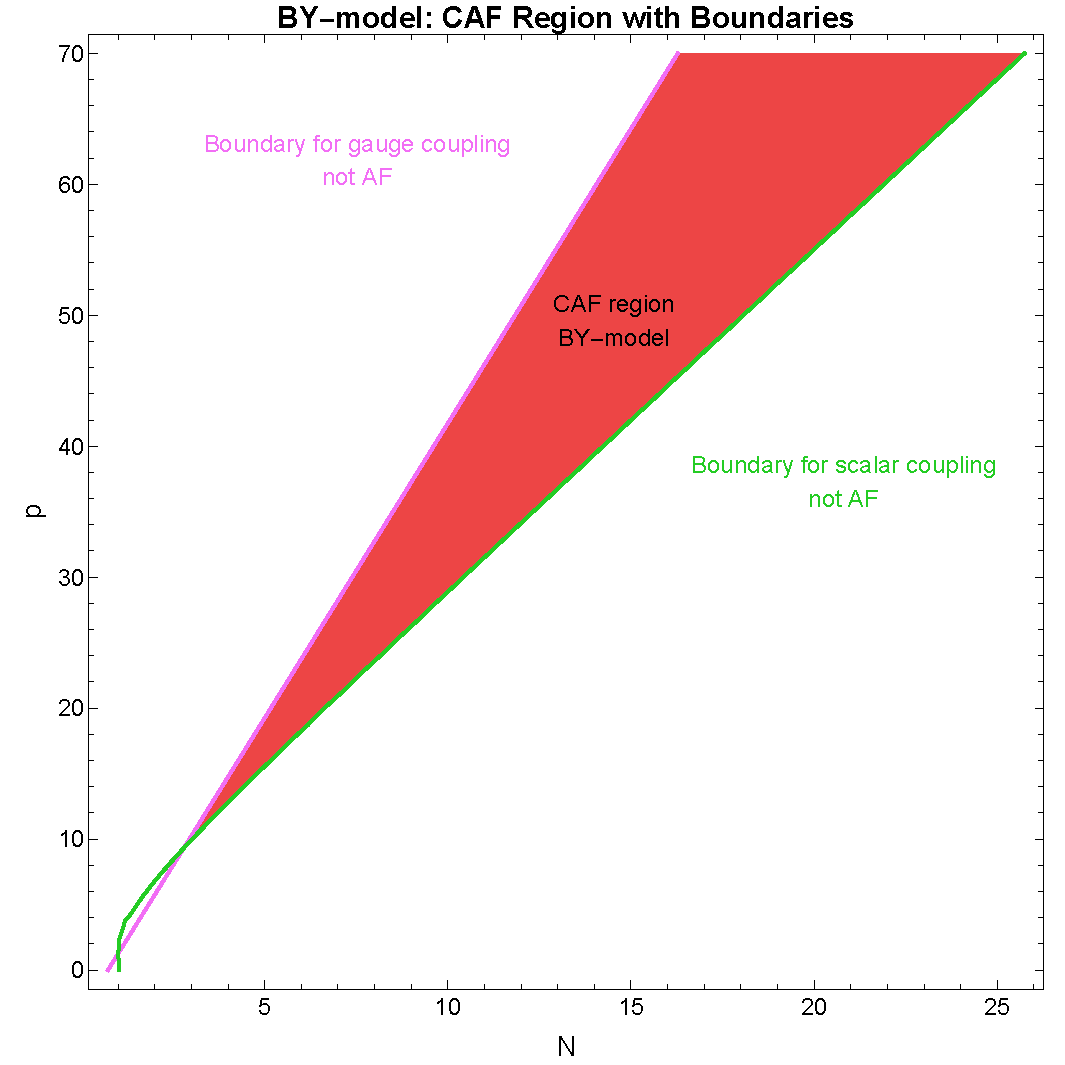
\includegraphics[width=0.6\textwidth]{Figures/boundaries.pdf}
    \caption{Figure displays the CAF region for the gauge and Yukawa coupling not on fixed flow, and which couplings lose asymptotic freedom at the lower boundary (Scalar coupling in green) and upper boundary (gauge coupling, pink).}
\label{fig:boundary}
\end{figure}
Now, a CAF analysis can be made on these models. Using the conditions mentioned in Equation \ref{eq:CAF} and \ref{eq:CAFfixed}, and the beta functions Equation \ref{eq:betagwithp}, \ref{eq:betaywithp}, and \ref{eq:betalamwithp}. In Figure \ref{fig:cafby}, the results of the CAF analysis are shown in the parameter space $(N,p)$. The dark region in both figures shows the conditions on the coefficients in the beta functions when the Yukawa and gauge couplings are not on fixed flow. That is, the Yukawa coupling becomes irrelevant when constraining the coefficients of the scalar couplings' beta function. This is because the gauge coupling will go slower to zero than the Yukawa. Both of these dark regions create a triangle, which does not extend to $p=0$, which fits with the results of the $p=0$ models. To better understand what couplings lose asymptotical freedom, see Figure \ref{fig:boundary}, which shows that the gauge coupling loses asymptotical freedom at too high p\footnote{Note that when the gauge coupling loses asymptotic freedom, so does the scalar and Yukawa coupling.}. So, the upper boundary is from the gauge coupling, and the lower boundary is from the scalar coupling. Another feature of the Figure \ref{fig:cafby} is the light blue region. This is the CAF conditions for when the Yukawa and gauge coupling are on fixed flow, i.e. the couplings go to zero at the same rate and thus neither coupling can be ignored. Note that the light blue region also expands underneath the dark blue region, so that the CAF space includes both regions for the case of the gauge and Yukawa coupling on fixed flow. It should further be noted that the CAF regions are possibly completely asymptotical, for the model to be CAF, the values of $\alpha_{y_0}$, $\alpha_{g_0}$, and $\alpha_{\lambda_0}$ are constrained as well (see Equation \ref{eq:CAFalpha} and \ref{eq:CAFalphafixed}). To better understand these conditions and these regions, flow diagrams have been made both within each region and outside of each region. 




The examples shown here are from the BY-model, but similar flow diagrams can be made for the GG-model. First, consider Figure \ref{fig:flowgy}. The left plot displays the gauge versus Yukawa coupling for $N=5$, $p=30$. This choice of the parameters puts the model outside of the CAF region, where the gauge coupling loses asymptotic freedom. The flow plot (with arrows pointing toward the UV) also shows that there is no region within the plot where the gauge coupling is asymptotically free. Further, one can see that for $\alpha_g=0$, the Yukawa coupling will diverge, hitting a Landau pole at UV. This is exactly as one would expect, since the gauge coupling is responsible for making the Yukawa coupling asymptotically free. Now consider the figure to the right in Figure \ref{fig:flowgy}, this is the same model with the same values of $N$ and $p$. The difference is that it shows the gauge versus the scalar coupling. As already concluded from the plot to the left, the gauge coupling cannot be asymptotically free. For a non asymptotically free gauge coupling, the scalar coupling cannot be asymptotically free\footnote{The assumption that $b_0<0$ is used in the CAF analysis regarding the scalar coupling. }. That the gauge coupling is not asymptotically free can also be seen on the flow plot to the right. Here, none of the arrows point towards the left, thus the gauge coupling cannot be asymptotically free. If we then consider the scalar coupling, we can see that none of the arrows point towards $\alpha_\lambda=0$. \comment{the green lines shouldn't be there}

In Figure \ref{fig:flowlam}, the case of $N=10,p=12$ is shown. These flow plots are below the dark blue region on Figure \ref{fig:cafby}, and are not asymptotically free for the scalar coupling in the case of the Yukawa coupling going to zero faster than the gauge coupling, as can be seen in Figure \ref{fig:boundary}. However, as mentioned earlier, Figure \ref{fig:boundary} shows that this is not within the CAF region for the scalar coupling. For the flow diagram to the left in Figure \ref{fig:flowlam}, a green dashed line can be seen, which shows the fixed flow of the gauge and Yukawa coupling. Everything underneath this line is asymptotically free in both couplings. Thus, the Yukawa and gauge coupling can be asymptotically free in this case. This flow diagram is shown in Figure \ref{fig:flowlam}. As seen on the flow plot to the right, where the gauge and scalar coupling is plotted for $N=10$, $p=12$ as well, for a positive scalar coupling, the flow always goes to infinity, and thus is not asymptotically free. For the region for $\alpha_\lambda<0$, which we are not interested in because it can create an unbounded potential from below, we see that the arrows actually point towards $\alpha_\lambda=0$, however, in the CAF analysis, we require a positive value of $\alpha_\lambda$ and thus no possible asymptotically free flow lines on this chart.

To compare more values of $N$ and $p$ to each other using flow diagrams figures \ref{fig:gridgy}, \ref{fig:gridlam} and \ref{fig:gridlamfixed}. Figure \ref{fig:gridgy} shows whether the gauge and Yukawa coupling are asymptotically free, where the asymptotically free values of $N$, $p$ have a green background colour, whereas the red colour shows that it is not asymptotically free in both couplings. The same values of $N$, $p$ are shown in the second grid in Figure \ref{fig:gridlam}, here the couplingspace is the gauge vs scalar coupling. The green here shows an asymptotically free scalar coupling, and the red background colour shows that the scalar coupling is no longer asymptotically free. Now, if we combine the knowledge from the two plots, the conclusion is that only (for this case) $N=10$, $p=30$ is CAF. Going back to Figure \ref{fig:cafby}, these values lie within the CAF region for the Yukawa and gauge coupling, not on fixed flow. So the two approaches give the same result. 


The other CAF region for Yukawa and gauge couplings on fixed flow can be checked similarly. The fixed flow changes nothing in the flow plots of the gauge versus Yukawa coupling. The flow plots for the scalar coupling, however, can be seen in Figure \ref{fig:gridlamfixed}. The three figures in the bottom left all look the same. Within the lines of fixed flow (of the scalar and gauge coupling), the arrows go downwards until they hit the lower fixed flow line. Then they move diagonally up toward orgio. This ensures that scalar couplings are indeed asymptotically free, as the green background colour also suggests between the two fixed flow lines. These three flow plots also have asymptotically free gauge coupling, since the flow goes toward the origin. The plot to the top right in Figure \ref{fig:gridlamfixed} shows non-asymptotic freedom, which can also be seen from none of the arrows going towards $\alpha_\lambda=0$, this is the case because the gauge coupling is not asymptotically free in this case.

Thus, putting the conclusions of figures \ref{fig:gridgy} and \ref{fig:gridlamfixed}, shows that the lower boundary that the scalar coupling made for the case of off fixed flow, is no longer present and therefore the gauge coupling alone constrains whether the model is CAF or not. This also fits with Figure \ref{fig:cafby}, where the fixed flow region now has lower boundaries. 

\comment{The fixed flow case does not have $\alpha_\lambda >0$ at all energy scales on the AF flows?}
\subsection{GG and BY models with Ng chiral families}
To further consider the GG- and BY-model with a scalar in the fundamental representation, we now consider more than one chiral family. To add more chiral families first the  

\section{Chiral models with scalars}
\subsection{GG-model with p=0}

\begin{equation}
    \text{SU}(N)\times \text{SU}(N-4)\times \text{U}(1)
\end{equation}
where the transformation of the scalar, anti-fundamental fermion, and two index antisymmetric fermion under each group is denoted in Table \ref{}.
To write the Lagrangian down, we need to ensure that all terms will be invariant under $U(1)$ and that no indices remains open. To do this we start by writing down the kinetic terms for all particles. Let us first consider the free theory:
\begin{equation}
    \mathcal{L}_{free}= i \bar \Psi_{ij}\sigma^\mu \partial_\mu\Psi_{ij}+i \bar \psi_i^a\sigma^\mu \partial_\mu\psi_i^a+\partial_\mu (\phi^*)_i\partial^\mu\phi_i\;,
\end{equation}
where $\sigma^\mu$ is used because the fermions are chiral and thus are massless. Next, we want to consider the interacting theory, which we do by promoting the global $U(1)$ symmetry of the Lagrangian to a local symmetry. To ensure that ... we introduce the covariant derivative $\partial_\mu \to D_\mu= \partial_\mu - ie(T^a)^i_{\,j}A_\mu^a$
\begin{equation}
    \mathcal{L}_{kinetic}= -\frac{1}{4} F_{\mu\nu}^a F^{\mu\nu\,a}+i \bar \Psi_{ij}\slashed{D}\Psi_{ij}+i \bar \psi_i^a\slashed{D}\psi_i^a+(D_\mu \phi^*D^\mu\phi)\;,
\end{equation}
where $F_{\mu\nu}^a=\partial_\mu A_\nu^a-\partial_\nu A_\mu ^a+g f^{abc}A_\mu^bA_\nu^c$, with $A_\mu$ being the connection. This gives us our first coupling constant, $g$. If we write out the first term, we obtain
\begin{equation}
    F_{\mu\nu}^a F^{\mu\nu\,a}\approx(\partial_\mu A_\nu^a)^2+ g f^{abc}(\partial_\mu A_\nu^a)A_\mu^bA_\nu^c +g^2 f^{abc}f^{def}A_\mu^bA_\nu^cA_\mu^dA_\nu^e\;,
\end{equation}
which gives us the gauge boson propagator and the two gauge bosons vertices
\comment{feynman diagrams}
The three remaining kinetic terms gives us the scalar and two fermion propagators 
\comment{feynman diagram}
Next, we consider all the possible interaction terms, which we can write in the Lagrangian. Consider first, the possible Yukawa interactions. Terms like $\Psi_{ij}\bar A_{ij}H^i$ and $\psi \bar \psi H^i$ are not invariant under $U(1)$. However, mixing the two fermion representations, is possible, this however gives an open gauge index from the anti-fundamental fermion. To fix this we take the coupling with the same gauge index, giving us $2a=2(N-4)$ Yukawa terms including the hermitian conjugated terms
\begin{equation}
    \mathcal{L}_{Yukawa}= y^a\Psi_{ij} \psi ^a_{\, i} H^j + h.c.\; ,
\end{equation}
Lastly, we have to consider possible quartic scalar terms. Again, ensuring $U(1)$ invariant terms, we can write terms like
\begin{equation}
    \mathcal{L}_{quartic}= 
    \lambda_1 (H^\dagger_i H_j)^2 
    + \lambda_2 (\bar \Psi_{ij}\Psi_{ij})^2
    +\lambda_3 (\bar \psi_{i}\psi_{j})^2
    +\lambda_4 (H^\dagger_i H_j)(\bar \psi_{i}\psi_{j})
    +\lambda_5 (H^\dagger_i H_j)(\bar \Psi_{ij}\Psi_{ij})
    +\lambda_2 (\bar \psi_{i}\psi_{j})(\bar \Psi_{ij}\Psi_{ij})
    +\lambda_2 (\bar \Psi_{ij}\Psi_{ij})^2+...\;,
\end{equation}
and similar terms. However, we will impose another condition namely that the theory needs to be renomalizablel. This means that the coupling, shouldn't have negative dimensions. The quartic scalar lagrangian thus simplifies to one term
\begin{equation}
    \mathcal{L}_{quartic}= 
    \lambda H^\dagger_i H_i H^\dagger_j H_j \;,
\end{equation}
thus we also have one scalar coupling, with the coupling constant $\lambda$. From the scalar and the yukawa terms we obtain three new vertices. The full Lagrangian thus reads
\begin{equation}
    \mathcal{L}= -\frac{1}{4} F_{\mu\nu}^a F^{\mu\nu\,a}+i \bar \Psi_{ij}\slashed{D}\Psi_{ij}+i \bar \psi_i^a\slashed{D}\psi_i^a+(D_\mu \phi^*D^\mu\phi)^2+(y^a\Psi_{ij} \psi ^a_{\, i} H^j + h.c.)+\lambda H^\dagger_i H_i H^\dagger_j H_j 
    \;.
\end{equation}

\subsubsection{Beta functions of the Lagrangian}
To analyze wether the theory is asymptotical free, we will use the Callan-Symanzik Equation \ref{h}. The beta function will first be computed for the gauge coupling
\begin{equation}
    \beta(\alpha_g)=\mu\frac{\text{d}\alpha_g}{\text{d}\ln\mu}= b_0 \alpha_g^2\;,
\end{equation}
where $\alpha_g=\frac{g^2}{4\pi}$ and $\mu$ is an arbitrary energy-scale. The beta equation for the gauge interaction can be computed by calculating the two, one-loop diagrams\comment{insert feynman diagrams that contribute}. To compute this we first need to renormalize the Lagrangian.  

For the gauge coupling the betafunction is thus (without scalars)
\begin{equation}
    \beta(g)=-\frac{g^3}{(4\pi)^2}\left[\frac{11}{3}C_2(G)-\frac{2}{6}T(R)\right]\;,
\end{equation}
This took quite a lot of computation, and I realized so would the remaning beta functions. I then chose to use a numerical approach, the beta function with scalars was then looked up:
\begin{equation}
    \beta(g)=-\frac{g^3}{(4\pi)^2}\left[\frac{11}{3}C_2(G)-\frac{2}{6}T(F)-\frac{1}{3}T(S)\right]\;,
\end{equation}

When computing the betafunction for the yukawa and the scalar coupling, the terms dependent on the Yukawa coupling is not completely trivial. They will have an index, because the coupling has the $a$ index, for the beta function of the Yukawa coupling
\begin{align}
    \beta_{y}\sim c_1g^2y_i + c_2 y^T \bar y y_i\;, 
\end{align} 
where the last term
\begin{equation}
    y^T \bar y =\sum_k^M y_k y_k^*=\sum^M_k |y_k|^2\;,
\end{equation}
for all Yukawas equal this reduces to
\begin{equation}
   \sum^M_k |y_k|^2=My^2\;,
\end{equation}
Only the terms with $y^3$ will be effected by the $M=N\pm4 +p$ factor. Thus, only the prefactors $c_2\to M c_2$,  $d_3\to M d_3$ and  $d_5\to M^2 d_5$. This however, does not change the CAF condition not on Fixed flow, hence none of the coefficients take part in the conidtions. However, for fixed flow condition the CAF conditions include all coefficients
\begin{align}
    &b_0<0,\quad\quad b_0-c_1>0,\quad\quad \left(b_0-d_2-Md_3\frac{b_0-c_1}{Mc_2}\right)^2-4d_1\left(d_4+M^2d_5\left(\frac{b_0-c_1}{Mc_2}\right)^2\right)\geq 0,\\&b_0-d_2- Md_3 \frac{b_0-c_1}{Mc_2}+\sqrt{\left(b_0-d_2 - Md_3 \frac{b_0-c_1}{Mc_2}\right)^2-4d_1\left(d_4+M^2d_5\left(\frac{b_0-c_1}{Mc_2}\right)^2\right)}>0\;.
\end{align}  
For these CAF conditions the additional factor of $M$ from the Yukawa coupling cancels out, and therefore does not effect wether the theory is CAF or not. 
\subsection{BY-model with p=0}
\begin{table}[h] 
    \centering 
    \begin{tabular}{|c|c|c|c|c|} \hline Fields & $[SU(N)]$ & $SU(N+4)$  & $U(1)$ \\ \hline $\chi$ & $\ytableausetup{boxsize=0.25cm}\begin{ytableau}{}\\{}\end{ytableau}$ & 1 & $N+4$ \\ $\psi$ & $\bar\square$ & $\bar\square$ & $-(N+2)$ \\ \hline $\phi$ & $\bar\square$ & 1  & -2 \\ \hline 
    \end{tabular} 
    \caption{ caption} 
    \label{tab:BYp0} 
\end{table}
Considering a chiral model with scalars, we now focus on the Bars-Yankielowicz model. As seen in table \ref{tab:BYp0}, the main difference from the GG model is that instead og having a two index antisymmetric representation, we have a two-index symmetric representation. That is the fermionic field $\chi_{ij}=\chi_{ji}$. The lagrangian is similar to the one of GG and can be expressed as
 \begin{align*}\mathcal{L}= -\frac{1}{4} F_{\mu\nu}^a F^{\mu\nu\,a}+i \bar \chi^{ij}\slashed{D}\chi_{ij}+i \bar \psi_{i\,a}\slashed{D}\psi_i^a+(D_\mu \phi^{*\,i})(D^\mu\phi_i)+(y^a\chi^{ij} \psi ^a_{\, i} \phi_j + h.c.)+\lambda (\phi^{\dagger}_i \phi^i)( \phi^{\dagger}_j \phi^j )
    \;.
 \end{align*}
There is another scalar quartic term however for (anti-)fundamental representations it is not linearly independent on the quartic scalar term in the lagrangian. Let us start by proving that 
\begin{align}
    (\phi_i^\dagger T_i ^{\,A\,j}\phi^j)(\phi_k^\dagger T_k ^{\,A\,l}\phi^l)\;,
\end{align}
where the generators $T^A$ upholds the Fierz identity
\begin{align}
    T_i ^{\,A\,j}T_k ^{\,A\,l}=\frac{1}{2}\left(\delta_i^{\,l}\delta_k^{\,j}-\frac{1}{N}\delta_i^{\,j}\delta_k^{\,l}\right) \;.
\end{align}
The Fierz identity can be shown to be true for fundamental representations of $SU(N)$ by considering \dots
The generators of $SU(N)$ can be written as $n\times n $ traceless Hermitian matricies $T^a$. The noramlisation of theses matricies is first defined to be 
\begin{equation}
      \text{tr}(T^a T^b)=\frac{1}{2}\delta^{ab}\;,
\end{equation}
using this we can write a general matrix $M$ as a linear combination of the identity matrix and the generators of the Lie algebra
\begin{equation}
      M=n_0 I+n_aT^a\;,
\end{equation}
where $n_0$ and $n_a$ are coefficients. Now let us take the trace on both sides and simplify using that $\tr(T^a)=0$ and $\tr(I)=N$
\begin{equation}
      \tr(M)=n_0 \tr(I)+n_a\tr(T^a)=n_0N\;.\label{eq:tr1}
\end{equation}
Next using the definition of the normalisation of the generators
\begin{equation}
      \tr(MT^b)=n_0 \tr(IT^b)+n_a\tr(T^aT^b)=\frac{n_b}{2}\;.\label{eq:tr2}
\end{equation}
Now using Equation \ref{eq:tr1,eq:tr2}, the constants $n_0,n_a$ can be replaced, and the matrix $M$ can be written as
\begin{equation}
      M=\frac{\tr(M)}{N} I+2\tr(MT^a)T^a\;,
\end{equation}
the matrix decomposition can be written in index notation
\begin{equation}
      M_{ij}=\frac{\tr(M)}{N} \delta_{ij}+2\tr(MT^a)T^a_{ij}\;,
\end{equation}
Using that it is in Euclidian space with the metric $\delta_{ij}$, the traces cab be simplified, and the lhs can be rewritten
\begin{equation}
      \delta_{jk}\delta_{il}M_{lk}=\frac{1}{N} \delta_{kl}M_{lk}\delta_{ij}+2\delta_{ln}M_{lk}T^a_{kn}T^a_{ij}\;,
\end{equation}
which can be simplified to 
\begin{equation}
      \delta_{jk}\delta_{il}=\frac{1}{N} \delta_{kl}\delta_{ij}+2T^a_{kl}T^a_{ij}\;,
\end{equation}
Isolating 
\begin{equation}
      T^a_{kl}T^a_{ij}=\frac{1}{2}\left(\delta_{jk}\delta_{il}-\frac{1}{N} \delta_{kl}\delta_{ij}\right)
\end{equation}
Inserting this back into the term gives us
\begin{align}
    \frac{1}{2} (\phi_i^\dagger \phi^j)(\phi_k^\dagger \phi^l)\left(\delta_i^{\,l}\delta_k^{\,j}-\frac{1}{N}\delta_i^{\,j}\delta_k^{\,l}\right)=\frac{1}{2}\left[\phi^{\dagger}_i \phi^j \phi^{\dagger}_j \phi^i-\frac{1}{N}\phi^{\dagger}_i \phi^i \phi^{\dagger}_k \phi^ik\right]=\frac{1}{2}\left(1-\frac{1}{N}\right) (\phi^{\dagger}_i \phi^i))^2\;,
\end{align}
so it is not linearly independt on the quartic term in the lagrangian. 
\subsection{Beta functions}
For the couplings defined as \comment{I need to have yi and alphai }
\begin{align*}
    \alpha_g = \frac{g^2}{(4\pi)^2}, \quad \alpha_y = \frac{y^2}{(4\pi)^2}, \quad\alpha_\lambda = \frac{\lambda}{(4\pi)^2}
\end{align*}
For GG model:
\begin{align}
    \beta_{\alpha_g}&=-\frac{11+18N}{3}\alpha_g^2\\
    \beta_{\alpha_y}&= \frac{\alpha_y }{2}\left[(3 N-1)
   \alpha_y+6 \alpha_g \left(-3 N+2+\frac 5N\right)\right]\\
    \beta_{\alpha_\lambda}&=\alpha_\lambda\left[2(N+1)\alpha_y-\frac{6 \alpha_g \left(N^2-1\right)}{N}+4 \alpha_\lambda (N+4)\right]-\frac{1}{2} (N+3)\alpha_y^2+\frac{3 \alpha_g^2 \left(N^3+N^2-4 N+2\right)}{4 N^2} 
\end{align}
For BY model:
\begin{align}
    \beta_{\alpha_g}&=-\frac{-13+18N}{3}\alpha_g^2\\
    \beta_{\alpha_y}&= \frac{\alpha_y}{2}\left[(3 N+5)\alpha_y+6 \alpha_g\left(-3 N-2+\frac 5N\right) \right]
   \\
   \beta_{\alpha_\lambda}&=\alpha_\lambda\left[2(N+1)\alpha_y-\frac{6 \alpha_g 
   \left(N^2-1\right)}{N}+4 \alpha_\lambda (N+4)\right]-\frac{1}{2} (N+3)
  \alpha_y^2+\frac{3 \alpha_g^2 \left(N^3+N^2-4 N+2\right)}{4 N^2} 
\end{align}
For large N both models reduce to
\begin{align}
    \beta_{\alpha_g}&\approx-6N\alpha_g^2\\
    \beta_{\alpha_y}&\approx N\alpha_y\left(-9\alpha_g+\frac{3}{2}\alpha_y\right)\\
    \beta_{\alpha_\lambda}&\approx N\left(\alpha_\lambda\left[2\alpha_y-6 \alpha_g 
   +4 \alpha_\lambda \right]-\frac{1}{2}
  \alpha_y^2+\frac{3}{4} \alpha_g^2 \right)
\end{align}
\subsection{GG and BY models with $p\neq0$}
\begin{table}[h]
    \centering
    \begin{tabular}{|c|c|c|c|c|c|}
    \hline
    Fields & $[SU(N)]$ & $SU(N - 4 + p)$ & $SU(p)$ & $U_1(1)$ & $U_2(1)$ \\
    \hline
    $\Psi$ & $\ytableausetup{boxsize=0.25cm}\begin{ytableau}{}\\{}\end{ytableau}$ & $1$ & $1$ & $N - 4$ & $2p$ \\

    $\tilde\psi$ & $\bar\square$ & $\bar\square$ & $1$ & $-(N - 2)$ & $-p$ \\

    $\psi$ & $\square$ & $1$ & $\square$ & $N - 2$ & $-(N - p)$ \\
    \hline
    $\phi$ & $\bar\square$ & $1$ & $1$ & $2$ & $-p$ \\
    \hline
    \end{tabular}
    \caption{GG model } 
    \label{tab:GGp} 
\end{table}


\begin{table}[h]
    \centering
    \begin{tabular}{|c|c|c|c|c|c|}
    \hline
    Fields & $[SU(N)]$ & $SU(N + 4 + p)$ & $SU(p)$ & $U_1(1)$ & $U_2(1)$ \\
    \hline
    $\chi$ & $\ytableausetup{boxsize=0.25cm}\begin{ytableau}{}&{}\end{ytableau}$ & $1$ & $1$ & $N + 4$ & $2p$ \\

    $\tilde\psi$ & $\bar\square$ & $\bar\square$ & $1$ & $-(N + 2)$ & $-p$ \\

    $\psi$ & $\square$ & $1$ & $\square$ & $N +2$ & $-(N - p)$ \\
    \hline
    $\phi$ & $\bar\square$ & $1$ & $1$ & $-2$ & $-p$ \\
    \hline
    \end{tabular}
    \caption{BY model } 
    \label{tab:BYp} 
\end{table}
A second set of models we will consider, is the GG- and BY-Model with $p\neq0$, we will see that these open of for CAF even if the yukawa and scalar coupling are not on fixed flow. First, the model considered is similar to the ones with $p=0$ i.e. having one scalar in the anti-fundamental representation. The transformation table changes a bit (see Table \ref{tab:GGp} and \ref{tab:BYp}), however the lagrangian will be similar
\begin{equation}
    \mathcal{L}= -\frac{1}{4} F_{\mu\nu}^a F^{\mu\nu\,a}+i \bar \Psi_{ij}\slashed{D}\Psi_{ij}+i \bar \psi_i^a\slashed{D}\psi_i^a+i \bar {\tilde \psi_i^a}\slashed{D}\tilde\psi_i^a+(D_\mu \phi^*D^\mu\phi)^2+(y^a\Psi_{ij} \tilde\psi ^a_{\, i} \phi^j + h.c.)+\lambda (\phi^\dagger_i \phi_i)^2 
    \;,
\end{equation}
where the kinetic term for the $\tilde\psi$ has been added. Only the one Yukawa term can be written down, for the lagrangian to be invariant under both $U_1(1)$ and $U_2(1)$. The beta functions of the models will aslo be similar to beta equations in Equation \ref{} and \ref{}. The only cahnge will be to the gauge beta function, because the amount of fermions effects the $b_0$ coefficient. Using the Equation \ref{}, we can compute the gauge beta function
\begin{equation}
    \beta(\alpha_g)=-{2\alpha_g^2}\left[\frac{11}{3}C_2(G)-\frac{2}{3}T(F)-\frac{1}{3}T(S)\right]\;,
\end{equation}
where $C_2(G)=N, \,T(F)_\Psi=\frac{N+2}{2},\, T(F)_\psi=\frac{1}{2},\, T(F)_{\tilde\psi}=\frac{1}{2},\, T(S)_\phi=\frac{1}{2}$ inserting this we obtain
\begin{equation}
    \beta(\alpha_g)=-{2\alpha_g^2}\left[\frac{22}{6}N-\frac{2}{3}\left(\frac{N\mp4+p}{2}+\frac{p}{2}+\frac{N\mp2}{2}\right)-\frac{1}{6}\right]\;,
\end{equation}
\begin{equation}
    \beta(\alpha_g)=-\frac{\alpha_g^2}{3}\left[18N-4p\pm{12}-1\right]\;,
\end{equation}
where the two remaining beta functions are given by
\begin{align}
    \beta_{\alpha_y}&= \frac{\alpha_y}{2}\left[(3 N+2\mp3)\alpha_y+6 \alpha_g\left(-3 N\pm2+\frac 5N\right) \right]
   \\
   \beta_{\alpha_\lambda}&=\alpha_\lambda\left[2(N+1)\alpha_y-\frac{6 \alpha_g 
   \left(N^2-1\right)}{N}+4 \alpha_\lambda (N+4)\right]-\frac{1}{2} (N+3)
  \alpha_y^2+\frac{3 \alpha_g^2 \left(N^3+N^2-4 N+2\right)}{4 N^2} 
\end{align}
where the top sign refers to the GG-model and the lower sign refers to the BY-model. 
\subsection{GG and BY models, new scalar representation, with $p\neq0$}
 
\section{Infinite heat order}
Before diving into the analysis of models with symmetry non-restoration at finite $N$, we first review the results of our previous paper \cite{Bajc:2021}. This work provided a much-needed UV completion for models of symmetry non-restoration, which historical models such as Weinberg's \cite{Weinberg:1974hy} lacked. To understand this mechanism, let us briefly review Weinberg's foundational setup. This model features two scalars and has a quartic potential with a cross-coupling term that preserves a discrete $\mathrm{Z}_2\times\mathrm{Z}_2$ symmetry:
\begin{equation}
    V=\frac{\lambda_1}{4}\phi^4_1+\frac{\lambda_2}{4}\phi_2^4-\frac{\lambda}{2}\phi_1^2\phi_2^2\;. \label{eq:VfromWeinberg}
\end{equation}
For the model to be viable, the potential has to be bounded from below, imposing constraints on the couplings
\begin{align}
    \lambda_{1,2}>0\quad,\quad \lambda^2<\lambda_1\lambda_2\,.
\end{align}
At high temperatures, the potential acquires a leading-order thermal correction
\begin{equation}
    \Delta V_T= \frac{T^2}{24}((3\lambda_1-\lambda)\phi_1^2 +(3\lambda_2-\lambda)\phi^2_2)\;,
\end{equation}
which for $\lambda>3\lambda_2$ will ensure that $\phi_2$ acquires a negative thermal mass, resulting in a non-zero VEV at high temperatures. However, as mentioned above, this model is not UV complete, since the required large cross-coupling increases with the energy scale, eventually reaching a Landau pole before the UV. 

In our previous work, we expanded this framework to UV-complete models. We can split the models considered into two main categories: asymptotically free or safe. In this paper, we focus on the models which are asymptotically free. Two branches of scalar models were considered. The first considers two singlet scalars coupled through fermions in the fundamental representation of $\mathrm{SU}(N_c)$ while also introducing a separate set of fermions that interact with the gauge fields but remain inert to the scalars (no Yukawa couplings) to provide additional freedom in the RGEs. This model was also generalised to a real scalar vector field $\phi$ with $d_\phi$ components. Both models were analysed near the UV, with a fixed-flow assumption, ensuring complete asymptotic freedom of all couplings and that they all scale as $1/t$ in the UV, where $t=\log(\mu/\mu_0)$ is the RG time. None of these models supported symmetry non-restoration at high energies. The models failed when requiring all the couplings to be on fixed flow, i.e.\ they could not both support complete asymptotic freedom and symmetry non-restoration. Therefore, we turned to a different set of asymptotically free models. 

In the second set of models, we extended the framework to include gauged scalars, meaning that the scalars were no longer singlets under the gauge group. First, models with one gauge group $ \mathrm{SU}(N_{c})$ were explored. This again resulted in symmetry restoration at high temperatures due to the high symmetry of the models, both for two and $N_s$ fundamental scalars. The result, however, changed when considering a product of two simple gauge groups $\mathrm{SU}(N_{c_1})\times\mathrm{SU}(N_{c_2})$. This model thus achieved enough mathematical freedom to satisfy both the fixed flow conditions and the negative thermal mass condition, resulting in symmetry non-restoration at high energies. 

Let us elaborate on this specific model. Each scalar $\varphi_i$ will be in the fundamental representation under its respective gauge group $\mathrm{SU}(N_{c_i})$ and a singlet under the other. The potential takes the form
\begin{align}
    V=\frac{\lambda_1}{2}\left(\vec{\varphi}_1^*\cdot\vec{\varphi}_1\right)^2+\frac{\lambda_2}{2}\left(\vec{\varphi}_2^*\cdot\vec{\varphi}_2\right)^2-
\lambda\left(\vec{\varphi}_1^*\cdot\vec{\varphi}_1\right)\left(\vec{\varphi}_2^*\cdot\vec{\varphi}_2\right)\;,
\end{align}
which is similar in structure to that of Weinberg's model \eqref{eq:VfromWeinberg} and includes the cross-coupling term between the two sectors, a crucial requirement for generating a negative mass squared.

To verify the presence of symmetry non-restoration, we first considered the effective potential $\Delta V_T$ at large $N_{c_i}$. In this process, we parameterised the couplings in terms of RG time to enforce the fixed flow solution. Further, the couplings were scaled by $N_{c_i}$ to ensure stable RGEs in the Veneziano limit of $N_{c_i}\to \infty$
\begin{align}
    g_i^2=\frac{16\pi^2\tilde\alpha_i}{N_{ci}t}\quad,\quad \lambda_i=\frac{16\pi^2\tilde\lambda_i}{N_{ci}t}\quad,\quad\lambda=\frac{16\pi^2\tilde\lambda}{\sqrt{N_{c1}N_{c2}}t}\;,
\end{align}
for $i=1,2$. We further introduced the variables $\tilde\lambda_\pm=\frac{1}{2}\left(\tilde\lambda_1\pm\tilde\lambda_2\right)$, and $\tilde\alpha_\pm=\frac{1}{2}\left(\tilde\alpha_1\pm\tilde\alpha_2\right)$. Using these variables, enforcing fixed flow trajectories, the RGEs yielded the following solutions
\begin{align}\label{eq:LO_sol}
    \tilde\alpha_-&=0 \;,\nonumber\\
\tilde\lambda_+&=\frac{6\tilde\alpha_+-1}{4}\;,\\
\tilde\lambda_-^2+\tilde\lambda^2&=\frac{1}{16}\left(24\tilde\alpha_+^2-12\tilde\alpha_++1\right)\;,\nonumber
\end{align}
which are valid for
\begin{align}
    \tilde\alpha_+\geq(3+\sqrt{3})/12\;.
\end{align}

From the effective potential $\Delta V_T$, the thermal mass parameters $\mu_1^2$ and $\mu_2^2$ are extracted. We then substituted the RG solutions into the thermal mass equation. Additionally, from the requirement of $\tilde\lambda>0$, we minimised the mass parameter with respect to $|\tilde\lambda|^2$. Doing so, we obtained the minimised mass parameter for $\varphi_1$
\begin{align}
    \mu_1^2=\frac{12\tilde\alpha_+-1}{2}-2\sqrt{\frac{24\tilde\alpha_+^2-12\tilde\alpha_++1}{16}}
\sqrt{1+\frac{N_{c2}}{N_{c1}}}\;.
\end{align}
The equation allows for a negative mass squared, because the ratio of the colours $\frac{N_{c_2}}{N_{c_1}}$ is a free parameter, it can be chosen sufficiently large such that the mass squared becomes negative. Thereby ensuring symmetry non-restoration at high temperatures. 

Checking the second condition for a potential bounded from below $\lambda_1\lambda_2-\lambda^2>0$ and ensuring real fixed flow solutions, we found a constraint on the ratio of the number of fermions to colours
\begin{align}
    \frac{1}{2}\left(2+3\sqrt{3}\right)\leq\frac{N_{fi}}{N_{ci}}<\frac{11}{2}\;.
\end{align}
Ultimately, this framework successfully yields a UV-complete model where one thermal mass turns negative for a given ratio $\frac{N_{c_2}}{N_{c_1}}$. At the same time, the ratio of fermions to colours is bounded to guarantee stability, equal gauge coupling $\tilde\alpha_1=\tilde \alpha_2$ and real RG solutions. All this effectively preserves the broken symmetry at high energies. 

Before moving on, note that this model also has an IR Banks-Zaks fixed circle. Previous analysis found that symmetry non-restoration could also be realised near this IR fixed point. It should also be noted that the previous work did identify more examples of negative mass squared at high energies. These examples include models featuring adjoint scalars within a similar gauge group structure $\mathrm{SU}(N_{c_1})\times\mathrm{SU}(N_{c_2})$ as well as asymptotically safe models. 

However, the analytical success of the model with two scalars, respectively gauged under $\mathrm{SU}(N_{c_1})\times\mathrm{SU}(N_{c_2})$ was achieved by simplifications of the Veneziano limit. This limit decpupled and simplified the RGEs. A critically relevant question is whether this characteristic of negative thermal mass persits beyond this limit. Thus, in the next section we will focus on finding a negative thermal mass for this model in the case of finite $N$. 

\section{\label{eqs} The 1-loop RG equations}
\subsection{\label{SUNc12} $SU(N_{c_1}) \times SU(N_{c_2})$  with two scalar fundamentals}

The model under consideration has the gauge symmetry $SU(N_{c_1}) \times SU(N_{c_2})$, 
where each scalar field $\varphi_i$ transforms in the fundamental 
representation of its respective $SU(N_{c_i})$ and is a singlet under the other. 
The most general potential is

\begin{align}
V=\frac{\lambda_1}{2}\left(\vec{\varphi}_1^*\cdot\vec{\varphi}_1\right)^2+\frac{\lambda_2}{2}\left(\vec{\varphi}_2^*\cdot\vec{\varphi}_2\right)^2-
\lambda\left(\vec{\varphi}_1^*\cdot\vec{\varphi}_1\right)\left(\vec{\varphi}_2^*\cdot\vec{\varphi}_2\right)\;.\label{eq:pot}
\end{align}

To derive the one-loop RGEs, we follow the approach established in \cite{Bajc:2021}, which maps different components of the RGEs onto different potential terms depending on the scalar potential. Since the model contains no Yukawa couplings, we only need the contributions $V_{\Lambda^2}$, $V_{\Lambda^S}$, and $V_{A}$ (Equation (A.20), (A.23), and (A.24) in \cite{Bajc:2021}) :
\begin{align}
\label{machacekhiggs}
16\pi^2\frac{d\lambda_{abcd}}{dt}=\Lambda^2_{abcd}+2\kappa\Lambda^Y_{abcd}-8\kappa H_{abcd}
-3g^2\Lambda^S_{abcd}+3g^4A_{abcd}
\end{align}
\begin{align}
    \label{VL2}
    V_{\Lambda^2}&\equiv\Lambda^2_{abcd}\frac{\phi^a\phi^b\phi^c\phi^d}{4!}
    =\frac{1}{2}\frac{\partial^2V}{\partial\phi^a\partial\phi^b}\frac{\partial^2V}{\partial\phi^a\partial\phi^b}\;,\\
    \label{VLS}
    V_{\Lambda^S}&\equiv-3g^2\Lambda^S_{abcd}\frac{\phi^a\phi^b\phi^c\phi^d}{4!}
    =-3g^2\phi^a\left(T^A(S)T^A(S)\right)_{ae}\frac{\partial V}{\partial\phi^e}\;,\\
    \label{VA}
    V_A&\equiv3g^4A_{abcd}\frac{\phi^a\phi^b\phi^c\phi^d}{4!}
    =\frac{3}{8}g^4\left(\phi^a\left\{T^A(S),T^B(S)\right\}_{ab}\phi^b\right)\left(\phi^c\left\{T^A(S),T^B(S)\right\}_{cd}\phi^d\right)\;.
\end{align}
For this model, the potential terms are
\begin{align}
    V_{\Lambda^2}&=&
    \left(\left(2N_{c_1}+8\right)\lambda_1^2+2N_{c_2}\lambda^2\right)\frac{1}{2}
    \left(\vec{\varphi}_1^*\cdot\vec{\varphi}_1\right)^2\nonumber\\
    &&+\left(\left(2N_{c_2}+8\right)\lambda_2^2+2N_{c_1}\lambda^2\right)\frac{1}{2}
    \left(\vec{\varphi}_2^*\cdot\vec{\varphi}_2\right)^2\\
    &&-\left(2\left(N_{c_1}\lambda_1+N_{c_2}\lambda_2\right)\lambda+2\left(\lambda_1+\lambda_2\right)\lambda-4\lambda^2\right)
    \left(\vec{\varphi}_1^*\cdot\vec{\varphi}_1\right)\left(\vec{\varphi}_2^*\cdot\vec{\varphi}_2\right)\;,\nonumber\\
    V_{\Lambda^S}&=&
    -6\frac{N_{c_1}^2-1}{N_{c_1}}g_1^2\left(\frac{\lambda_1}{2}\left(\vec{\varphi}_1^*\cdot\vec{\varphi}_1\right)^2
    -\frac{\lambda}{2}\left(\vec{\varphi}_1^*\cdot\vec{\varphi}_1\right)\left(\vec{\varphi}_2^*\cdot\vec{\varphi}_2\right)\right)\nonumber\\
    &&
    -6\frac{N_{c_2}^2-1}{N_{c_2}}g_2^2\left(\frac{\lambda_2}{2}\left(\vec{\varphi}_2^*\cdot\vec{\varphi}_2\right)^2
    -\frac{\lambda}{2}\left(\vec{\varphi}_1^*\cdot\vec{\varphi}_1\right)\left(\vec{\varphi}_2^*\cdot\vec{\varphi}_2\right)\right)\;,\\
    V_{A}&=&\frac{3}{4}g_1^4\frac{N_{c_1}^3+N_{c_1}^2-4N_{c_1}+2}{N_{c_1}^2}
    \left(\vec{\varphi}_1^*\cdot\vec{\varphi}_1\right)^2\nonumber\\
    &&+\frac{3}{4}g_2^4\frac{N_{c_2}^3+N_{c_2}^2-4N_{c_2}+2}{N_{c_2}^2}
    \left(\vec{\varphi}_2^*\cdot\vec{\varphi}_2\right)^2\;.
\end{align}

To ensure that all the couplings are asymptotically free, i.e., that the model exhibits complete asymptotic freedom (CAF), we parametrise the couplings with a factor $1/t$ 
\begin{align}
i=1,2&:&g_i^2=\frac{16\pi^2\tilde\alpha_i}{N_{c_i}t}\quad,\quad \lambda_i=\frac{16\pi^2\tilde\lambda_i}{N_{c_i}t}\quad,\quad\lambda=\frac{16\pi^2\tilde\lambda}{\sqrt{N_{c_1}N_{c_2}}t}\;.
\end{align}
This ensures that the couplings all vanish at the same rate in the UV, a behaviour known as fixed-flow \cite{Giudice:2015}. With this parametrisation, the RGEs reduce to a set of coupled polynomial equations. Real solutions of these algebraic equations correspond to models exhibiting CAF, as long as the gauge coupling is asymptotically free, $b_0>0$. For the model to be physical viable it must also satisfy \eqref{eq:Vbounded} such that its potential is bounded from below. 

\begin{comment}
\noindent
Using the definition $N_{c_1} = x\,N_{c_2}$ and Equation (A.18) in \cite{Bajc:2021} the RGEs are given by 
\begin{align}\label{eq:finiteNRG}
-\tilde{\lambda}_1 \;=&\;
\left(2+\frac{8}{x N_{c_2}}\right)\tilde{\lambda}_1^{\,2}
+2\,\tilde{\lambda}^{\,2}
-6\!\left(1-\frac{1}{x^{2}N_{c_2}^{2}}\right)\tilde{\alpha}_1\tilde{\lambda}_1
\nonumber\\&+\frac{3}{2}\tilde{\alpha}_1^{\,2}\!\left(
1+\frac{1}{x N_{c_2}}-\frac{4}{x^{2}N_{c_2}^{2}}+\frac{2}{x^{3}N_{c_2}^{3}}
\right),\nonumber
\\[4pt]
-\tilde{\lambda}_2 \;=&\;
\left(2+\frac{8}{N_{c_2}}\right)\tilde{\lambda}_2^{\,2}
+2\,\tilde{\lambda}^{\,2}
-6\!\left(1-\frac{1}{N_{c_2}^{2}}\right)\tilde{\alpha}_2\tilde{\lambda}_2
\nonumber\\&+\frac{3}{2}\tilde{\alpha}_2^{\,2}\!\left(
1+\frac{1}{N_{c_2}}-\frac{4}{N_{c_2}^{2}}+\frac{2}{N_{c_2}^{3}}
\right),
\\[4pt]
-\tilde{\lambda} \;=&\;
\tilde{\lambda}\Bigg[
-\frac{4}{N_{c_2}\sqrt{x}}\,\tilde{\lambda}
+2\!\left(1+\frac{1}{x N_{c_2}}\right)\tilde{\lambda}_1
+2\!\left(1+\frac{1}{N_{c_2}}\right)\tilde{\lambda}_2
\nonumber\\&-3\!\left(
\tilde{\alpha}_1\!\left(1-\frac{1}{x^{2}N_{c_2}^{2}}\right)
+\tilde{\alpha}_2\!\left(1-\frac{1}{N_{c_2}^{2}}\right)
\right)
\Bigg] \ , \nonumber
\end{align}
\end{comment}
\noindent
The finite-$N$ RG equations we need to solve for this model take the form presented in eq.s \eqref{eq:finiteNRG}. Plugging in those the coupling redefinitions \eqref{eq:couplings} and solving perturbatively order by order, we have that the LO couplings must satisfy the system
\begin{align}
-\tilde\lambda^{(0)}_1&=&2\tilde\lambda^{(0)2}_1+2\tilde\lambda^{(0)2}-6\tilde\alpha^{(0)}_1\tilde\lambda^{(0)}_1+\frac{3}{2}\tilde\alpha_1^{(0)2}\;,\\
-\tilde\lambda^{(0)}_2&=&2\tilde\lambda_2^{(0)2}+2\tilde\lambda^{(0)2}-6\tilde\alpha^{(0)}_2\tilde\lambda^{(0)}_2+\frac{3}{2}\tilde\alpha_2^{(0)2}\;,\\
-\tilde\lambda^{(0)}&=&2\left(\tilde\lambda^{(0)}_1+\tilde\lambda^{(0)}_2\right)\tilde\lambda^{(0)}-3\left(\tilde\alpha^{(0)}_1+\tilde\alpha^{(0)}_2\right)\tilde\lambda^{(0)}\; ,
\end{align}
which is the system solved for the infinite-$N$ case in \cite{Bajc:2021}.  The NLO couplings will need to satisfy on the other hand the system
\begin{equation}\label{eq:NLORGeqp}
    \begin{split}
        &39\tilde\alpha_+^{(0)2}+(1-4\tilde\lambda_-^{(0)})^2-12\tilde\alpha_+^{(0)}(1-4\tilde\lambda_-^{(0)})+x\Big[1+39\tilde\alpha_+^{(0)2}+6\tilde\alpha_+^{(1)2}+16\tilde\lambda^{(0)}\tilde\lambda^{(1)}\\
        &-12\tilde\alpha_+^{(0)}\Big(1+2\tilde\alpha_+^{(1)}+4\tilde\lambda_-^{(0)}\Big)+8\tilde\lambda_-^{(0)}\Big(1-3\tilde\alpha_-^{(1)}+2\tilde\lambda_-^{(0)}+2\tilde\lambda_-^{(1)}\Big)\Big]=0 \ \ \ ,
    \end{split}
\end{equation}
\begin{equation}\label{eq:NLORGeqm}
    \begin{split}
        &39\tilde\alpha_+^{(0)2}+(1-4\tilde\lambda_-^{(0)})^2-12\tilde\alpha_+^{(0)}(1-4\tilde\lambda_-^{(0)})-x\Big[1+39\tilde\alpha_+^{(0)2}+6\tilde\alpha_-^{(1)2}\Big(4\tilde\alpha_+^{(0)}-1\Big)\\
        &-12\tilde\alpha_+^{(0)}\Big(1+4\tilde\lambda_-^{(0)}\Big)+8\tilde\lambda_-^{(0)}\Big(1+3\tilde\alpha_+^{(1)}+2\tilde\lambda_-^{(0)}-2\tilde\lambda_+^{(1)}\Big)\Big]=0 \ \ \ ,
    \end{split}
\end{equation}
\begin{equation}\label{eq:NLORGeq3}
    \begin{split}
        &-1+6\tilde\alpha_+^{(0)}-8\sqrt{x}\tilde\lambda^{(0)}+4\tilde\lambda_-^{(0)}+x\Big(-1+6\tilde\alpha_+^{(0)}-12\tilde\alpha_+^{(1)}-4\tilde\lambda_-^{(0)}+8\tilde\lambda_+^{(1)}\Big)=0 \ \ \ .
    \end{split}
\end{equation}


\noindent
The thermal effective potential is given by
\begin{align}
\Delta V_T=
\frac{T^2}{48}\sum_{i=1}^2\sum_{a=1}^{N_{c_i}}\left(4\frac{\partial^2V}{\partial\varphi_i^a\partial\varphi_{ia}^*}
+6g_i^2\frac{N_{c_i}^2-1}{N_{c_i}}\varphi_i^a\varphi_{ia}^*\right)\;,
\end{align}
which for the potential \eqref{eq:pot} yields
\begin{align}
\Delta V_T=
(4\pi)^2\frac{T^2}{24\log{T}}&\left(\left(2\left(\tilde\lambda_1-\sqrt{\frac{N_{c_2}}{N_{c_1}}}\tilde\lambda\right)
+3\tilde\alpha_1 \left(1 - \frac{1}{N_{c_1}^2} \right)
\left(\vec{\varphi}_1^*\cdot\vec{\varphi}_1\right)\right.\right.\nonumber\\
&\left.+\left(2\left(\tilde\lambda_2-\sqrt{\frac{N_{c_1}}{N_{c_2}}}\tilde\lambda\right)+3\tilde\alpha_2 \left(1 - \frac{1}{N_{c_2}^2} \right)\right)
\left(\vec{\varphi}_2^*\cdot\vec{\varphi}_2\right)\right)\;.
\end{align}

